\documentclass{lkx_thesis}
\usepackage{lkx_thesis}
\usepackage{lkx_diagrams}

\title{Exotic Spheres}
\subtitle{A Geometric Perspective}
\author{Lev Kruglyak}

\department{The Department of Mathematics}
\degree{Bachelor of Arts with Honors}
\subject{Mathematics}

\university{Harvard University}
\location{Cambridge, Massachusetts}
\date{April 2025}

\titlegraphic{graphics/title/e8.jpg}

\advisor{Dr. Stephen McKean}
\advisor{Professor Michael Hopkins}

\begin{document}

\makeatletter
{
	\begin{titlepage}
		\begin{center}
			\hfill
			\vfill
			{\Huge\scshape{\@title}}\\[2ex]
			{\Large\@subtitle}\\[0.5in]

			\includegraphics[width=3in]{\@titlegraphic}\\[0.5in]

			{\scshape

			{by\\[1em]}
			{\large\scshape{\@author}}\\[1em]
			{advised by\\[1em]}
			{\large\scshape\advisorlist}\\[0.5in]

			{A thesis presented to \\[1em]}
			% {\bfseries\large\textsl{\@university}\\[1em]}
			{\large\scshape{\@university}\\[1em]}
			in partial fulfillment of the\\
			requirements for the degree of\\[1em]

			{
			\large
			% {\bfseries\textsl\@degree}\\
			{\scshape\@degree}\\
			in the subject of
			% {\bfseries\textsl\@subject}\\[1em]
			{\scshape\@subject}\\[1em]
			}
			%
			% {\@location}\\
			% {\@date}\\
			}
			\vfill
		\end{center}
	\end{titlepage}
}
\makeatother
\pagebreak


\lkxtoc

\chapter*{Prologue}\label{chap:prologue}
\addcontentsline{toc}{chapter}{Prologue} 
% Epigraph
\begin{flushleft}
	\textsl{Existence plays a mischievous game with us,}\\
	\textsl{as though to tease and provoke us. In the }\\
	\textsl{midst of knowledge there yet again arises }\\
	\textsl{the mystery; in the midst of contemplation}\\
	\textsl{the riddle gains new strength.}\\
	\rule[0pt]{19.5em}{0.5pt}\\
	-- \textsc{Joseph Soloveitchik}\\
	% \phantom{-- }\textsl{``Ish ha'Halakhah''}
	\vspace{2em}
\end{flushleft}

% \begin{flushleft}
% 	\textsl{One might say that, in whatever manner God might have}\\
% 	\textsl{created the world, it would always have been in accordance}\\
% 	\textsl{with a certain general order. But God has chosen the most}\\
% 	\textsl{perfect world, that is, the one which is at the same time}\\
% 	\textsl{the simplest in hypothesis and richest in phenomena.}\\
% 	\rule[0pt]{26em}{0.5pt}\\
% 	-- \textsc{Gottfried Leibniz}\\
% 	% \phantom{-- }\textsl{``Discours de m\'etaphysique''}
% 	\vspace{2em}
% \end{flushleft}

Before talking about exotic spheres, I want to talk about symmetry.

% Projective plane analogy with torsion (Z/2 vs Z/28)

% Humanity has been fascinated by questions of physical space for thousands of years. As with many areas of math, this burning curiosity first arose in antiquity out of practical concerns: measuring the volume of a cylindrical grain silo, computing the circumference of the earth, predicting the motion of celestial bodies, etc. In order to make these questions precise in the idealized world of mathematical forms, we must first make our intuitive notions of space precise. 
% Euclidean geometry, for instance, takes place on an infinite continuum of points, and comes with a way to measure distances and angles. It also contains a strong notion of parallelism -- starting at a point and choosing a direction gives a straight line which extends indefinitely. If we pick any other point not this line, travelling in that same direction gives us a parallel, non-overlapping line.
%
% To us, physical space at the scales which we inhabit is so intuitively Euclidean, and so baked into the very structures of our mind that it's difficult to imagine where our assumptions might be biased. We tend to think of space as infinite and flat, just as Euclid's axioms describe. At the scale of daily life this is an accurate model, but at the scale of the Earth it completely falls apart. The Earth is neither infinite nor flat, and \emph{any} straight line path will eventually bring you back to your starting point. 
% And that's only the two-dimensional surface of the spherical Earth. What if the universe itself was finite, curving in on itself rather than extending indefinitely? You might imagine zooming into the depths of the cosmos with a super-powered telescope only to see familiar galaxies, and eventually Earth itself peering back at you.
% Even worse, what if space was non-orientable? Not only could flying in a straight path bring you right back to where you started, but you would find that upon your arrival the very notions of right and left seem to have swapped places -- as though you've entered a mirror world. All languages become illegible to you since they are now backwards from your perspective, a birthmark which used to be on the left side of your face appears to everyone else to be on your right. Only another trip along the same course you originally took is able to flip everything back.
%
% \begin{figure}
% 	\centering
% 	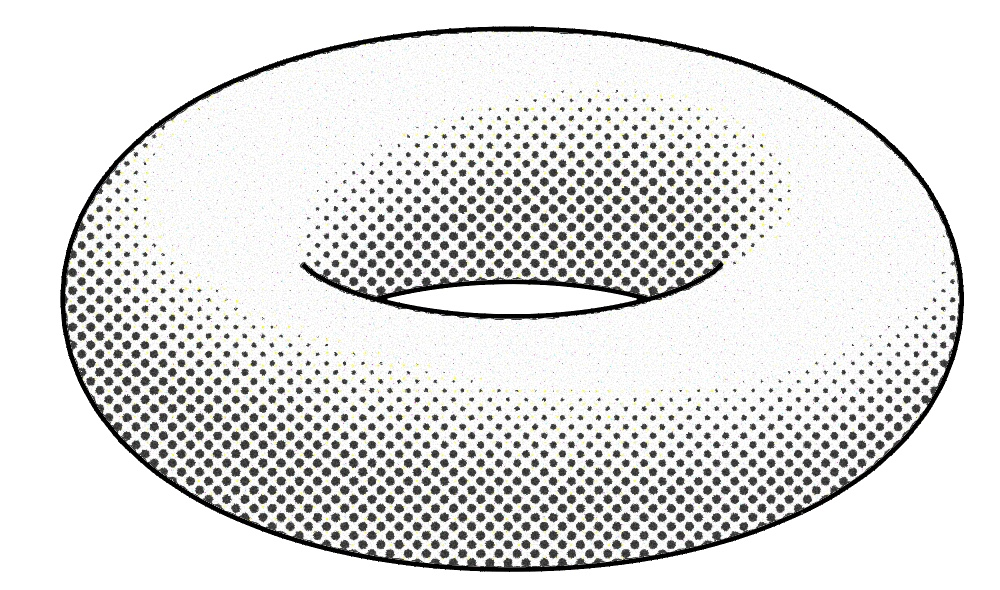
\includegraphics[scale=0.3]{graphics/diagrams/torus_non_vanishing_vector_field/result.jpg}
% 	\vspace{1em}
% 	\caption{A torus.}
% \end{figure}
%
% By relaxing our assumptions about the shape of space, geometry begins to quickly fill up with many such counter-intuitive non-Euclidean spaces and they find applications in unexpected places. Take for instance 
%
% \hspace{1em}
% % Many such axiomatic foundations exist, and lead 
%
% Let's start with the simple case of Euclidean space (think of a plane for instance) by describing some of its essential aspects. First and foremost Euclidean space is comprised of infinitely many points which \emph{extend continuously}, which informally means that Euclidean space is equipped with a qualitative concept of ``closeness''. Among other things, this 
%
% Euclidean space also comes with the stronger, quantitative notion of closeness -- this is known as \defn{distance}. A distance metric assigns to each pair of points a non-negative real number.

% \pagebreak

% \todo{The geometries they worked in were mostly flat, i.e. Euclidean and they relied on entirely (analytical?) methods to derive spatial relationships}
%
% \todo{Take a step back and see what data we have.}
%
% Classical geometry works in affine space, so we have: continuity of space, distance,  translation and homotethy. Translation gives us a global parallelism.
%
% Introduction of curvature
%
% Intrinstic  geometry via Theorema Egregium
%
% Symplectic manifolds, spin manifolds -> corresponding to physics
%
% Ehrlangen program

% At the scales they worked at, reality was best modelled by a plane or a (flat) three dimensional space.

% Homotopy classes of spaces
%
% PL manifolds
%
% During my last summer before graduating college, I went with some friends on a mountaineering trip up Banner peak, a picturesque mountain in the eastern Sierra Nevada range of California. 
% %
% % As we descended the glacier towards our base camp, ice axes in hand, I 
% So how \emph{do} we study objects which we can't touch, see, or possibly hope to visualize in their full complexity?
%
% There are two levels to understanding.
% \begin{enumerate}
% 	\item First, we
% \end{enumerate}
%
% Understanding an object by how it behaves with respect to other objects.
% \todo{spectral lines of atoms}
%
% One of the earliest methods to ``fingerprint'' topological objects was discovered by Euler.

% \cite{hatcher2002}


\chapter*{Conventions}\label{chap:conventions}
\addcontentsline{toc}{chapter}{Conventions} 
\chapter*{Conventions}

\subsection*{General}

\begin{itemize}
  \item Definitions of terms will be formatted {\color{blue}\emph{blue and emphasized}}, and hyperlinks will be formatted just blue (e.g. \cref{fig:first}).
  \item We use $\cong$ instead of $\oldcong$ to denote isomorphisms, diffeomorphisms, etc.
\end{itemize}

\subsection*{Algebra}

\begin{itemize}
  \item The group of units in a ring $A$ is denoted $A^\times$.
  \item A \defn{graded ring} is a ring $A$ equipped with a decomposition of its underlying group as $A=\bigoplus_{k\in \Z_{\geq 0}} A[k]$ such that the ring multiplication sends $A[k_1]\times R[k_2] \to A[k_1+k_2]$. Elements belonging to $A[k]$ are said to be \defn{homogeneous of degree $k$}[homogeneous element of a graded ring]. 
  \item A graded ring is said to be \defn{graded-commutative} if for any homogeneous elements $x\in A[k_1]$ and $y\in A[k_2]$, we have
    \[
      x\cdot y = (-1)^{k_1k_2} y\cdot x
    \]
  \item The \defn{completion}[completion of a graded ring] of a graded ring $A$ is the direct product $\widehat{A} = \prod_{k\geq 0} A[k]$.
  \item When expanding an element $a$ in a graded ring or completion of a graded ring as an infinite series, we use the notation
  \[
      a = a_0 + a_1t+a_2t^2+\cdots
  \]
  The variable $t$ should be understood as a notational formal variable.
  \item $A_{(1)}\subset A^\times$ denotes the units with monic leading coefficient (i.e. $a_0=1$).
\end{itemize}

\subsection*{Differential Topology}
\begin{itemize}
  \item A \defn{topological manifold} $M$ is a locally Euclidean second-countable Hausdorff space. \todo{boundary}
  \item A \defn{smooth structure} $\mathscr{S}$ on a topological manifold $M$ is a collection of open charts $\mathscr{S}=\{(U_\alpha, \varphi_\alpha)\}_{\alpha\in I}$ such that the transition functions 
	\begin{equation}\label{eq:transition-function}
		\lkxfunc{g_{\alpha\beta}}{\varphi(U_\alpha\cap U_\beta)}{\R^n\textrm{ or } \R^{n-1}\times [0,\infty)}
	\end{equation}
	are smooth for all $\alpha,\beta\in I$. We require that $\mathscr{S}$ be maximal with respect to this property, i.e. the addition of any chart $(U,\varphi)$ not in $\mathscr{S}$ breaks the smoothness of \cref{eq:transition-function}.
  \item Unless otherwise specified, all manifolds are assumed to be smooth, connected, and possibly with boundary. A \defn{closed}[closed manifold] manifold is a compact manifold with empty boundary.
  \item When introducing a manifold, we often put its dimension as a superscript. For example, ``let $M^n$ be a manifold'' should be read as ``let $M$ be an $n$-dimensional manifold''.

  \item We assume that all submanifolds $N\subset M$ are properly embedded and neat, i.e.
    \vspace{-0.5em}
    \begin{itemize}
      \item the inclusion $\iota : N \to M$ is a proper map,
      \item $\partial N\subset \partial M$,
      \item the boundary $\partial N$ intersects $\partial M$ transversally.
    \end{itemize}
\end{itemize}

\subsection*{Algebraic Topology}
\begin{itemize}
  \item Given a coefficient ring $R$, $\H^i(-; R)$ denotes the singular cohomology with coefficients in $R$, and $\H_i(-;R)$ denotes singular homology with coefficients in $R$. $\H^\bullet(-;R)$ is the singular cohomology ring.
  \item $\HdR$ denotes de-Rham cohomology, and $\Hc$ denotes compactly-supported de-Rham cohomology.
  \item Whenever we refer to a general (co)homology theory $h$, we mean one of the pairs:
    \begin{itemize}
      \item Singular (co)homology with coefficients in $R=\Z, \Z/2, \Z[1/2],$ or $\Q$.
      \item Compactly supported de-Rham cohomology and de-Rham cohomology.
    \end{itemize}
    The homology groups are denoted $h_i(-)$ and the cohomology groups are denoted $h_i(-)$. Note that all pairs 
\end{itemize}

\subsection*{Differential Geometry}
\begin{itemize}
  \item Vector bundles are over a field $\F=\R$ or $\C$, by default assumed to be $\R$.

  \item By default, we denote the total space of a vector bundle with normal math font, i.e. $E \to X$, and denote the bundle itself with calligraphic font, i.e. $\mathcal{E} : E \to X$. 

  \item The tangent bundle of a manifold $M$ is dented $\TT M$, with total space $\T M$.

  \item As with manifolds, a superscript $\mathcal{E}^k$ on a vector bundle denotes its rank. 

  \item Given a Riemannian inner product structure $\langle-,-\rangle$ on a vector bundle $\mathcal{E}^k$, we let $\S(\mathcal{E})$ be the associated sphere bundle (with fibers $S^{k-1}$) and $\D(\mathcal{E})$ the associated disk bundle (with fibers $D^k$). The total spaces of these bundles are
  \[
    \S(E) = \{ \xi\in E \mid \langle \xi, \xi\rangle =1 \}
    \quad\textrm{and}\quad
    \D(E) = \{ \xi\in E \mid \langle \xi, \xi\rangle\leq 1 \}
  \]
  respectively. Note that $\partial \D(E) = \S(E)$ as manifolds.
\end{itemize}


\chapter{Introduction}\label{chap:introduction}
% \begin{flushleft}
% 	\textsl{There is geometry in the humming of the strings,}\\
% 	\textsl{and there is music in the spacing of the spheres.}\\
% 	\rule[0pt]{21em}{0.5pt}\\
% 	-- \textsc{Pythagoras}\\
% 	\vspace{2em}
% \end{flushleft}

\begin{flushleft}
	\textsl{God created the integers,}\\
	\textsl{the rest is the work of man.}\\
	\rule[0pt]{13em}{0.5pt}\\
	-- \textsc{Leopold Kronecker}\\
	\vspace{2em}
\end{flushleft}

\todo{introduce, motivate, provide historical context.}

\begin{conjecture}[Poincar\'e Conjecture]
	Every closed topological $3$-manifold which is simply connected is homeomorphic to the $3$-sphere $S^3$.
\end{conjecture}

\begin{definition}
	If $U\subset \R^n$ is an open subset, a function $f : U \to \R^m$ is said to be \defn{smooth}[smooth function] if all partial derivatives of $f$ exist to all orders.
\end{definition}

\begin{definition}
	A \defn{smooth structure} $\mathscr{S}$ on a topological manifold $M$ (possibly with boundary) is a collection of charts $\mathscr{S}=\{(U_\alpha, \varphi_\alpha)\}_{\alpha\in I}$ such that the transition functions
	\begin{equation}\label{eq:transition-function}
		\lkxfunc{\varphi_\alpha\varphi_\beta^{-1}}{\varphi(U_\alpha\cap U_\beta)}{\R^n\textrm{ or } \R^{n-1}\times [0,\infty)}
	\end{equation}
	are smooth for all $\alpha,\beta\in I$. We require that $\mathscr{S}$ be maximal with respect to this property, i.e. the addition of any chart $(U,\varphi)$ not in $\mathscr{S}$ breaks the smoothness of \cref{eq:transition-function}.
\end{definition}
% A smooth structure gives rise to tangent spaces -- at each point of the3manifold there is a notion of infinitesimal direction, and the set of all such infinitesimal directions forms a vector space of tangent vectors. \todo{physics}

While the class of smooth manifolds offers a tempting for context for the exploration of the shape of space, it is far from the only type of manifold one can define. Another equally valid category in which to study topology of manifolds is $\Pl$, or the piecewise linear category. A $\Pl$ structure on a manifold consists of

\begin{conjecture}[Generalized Poincar\'e Conjecture]
	Letting $\mathscr{C}$ be either $\Top$, $\Pl$, or $\Diff$, any $\mathscr{C}$-manifold which is homotopy equivalent to the $n$-sphere $S^n$ is also $\mathscr{C}$-isomorphic to $S^n$.
\end{conjecture}

\begin{conjecture}[Hauptvermutung]
	\todo{this}
\end{conjecture}

\todo{questions about equivalence of TOP, PL, and DIFF}

\todo{goal of this chapter is provide some fundamental concepts needed to begin working on the problem}

\subsection{Morse Theory}

While a fully comprehensive introduction to Morse theory is outside of the scope of this thesis, we'll include a basic overview for completeness. A great classical introduction to Morse theory can be found in Milnor's book on the subject \cite{milnor1963morse}.

If $f : M \to \R$ is a smooth function on a manifold $M$, the points $p\in M$ where the differential $df_p : \T_p M \to \T_{f(p)} \R = \R$ vanish are known as \defn{critical points}, and their images in $\R$ are called \defn{critical values}. In terms of local coordinates $\{x^1,\ldots, x^n\}$ at $p$, this means that
\[
	\frac{\partial f}{\partial x^1}=\cdots=\frac{\partial f}{\partial x^n} = 0.
\]
A critical point $p\in M$ is said to be \defn{non-degenerate}[non-degenerate point] if the matrix
\[
	\everymath={\displaystyle}
	\renewcommand*{\arraystretch}{2}
	H_f(p) = \begin{pmatrix}
		\frac{\partial^2 f}{\partial x^1\partial x^1} & \cdots &
		\frac{\partial^2 f}{\partial x^1\partial x^n}                   \\
		\vdots                                        & \ddots & \vdots \\
		\frac{\partial^2 f}{\partial x^n\partial x^1} & \cdots &
		\frac{\partial^2 f}{\partial x^n\partial x^n}                   \\
	\end{pmatrix}(p)
\]
is invertible at $p$. This is called the \defn{Hessian matrix} of $f$ at $p$, and in this formulation depends on our chosen coordinate system.
There is a coordinate independent way to define the Hessian as a symmetric bilinear form on $\T_p M$ which makes the coordinate invariance of the condition of non-degeneracy manifestly apparent.

\begin{definition}
	The \defn{index}[index of a function] of $f$ at a point $p$ is the maximal dimension of a subspace on which $H_f(p)$ is negative definite, i.e. it is the dimension of $\{v\in \R^n \mid v^\intercal H_f(p) v < 0\}.$
\end{definition}

The index of a function at a point essentially describes the ``shape'' of the function out of a list of finitely many possible shapes. Remember, the index of a function on an $n$-dimensional manifold must be an integer between $0$ and $n$. For instance, in the case of a surface there are three possible shapes -- when both coordinates curve up we get a bowl facing up, when one curves up and one curves down we get a saddle, and when both coordinates curve down we get a bowl facing down. These shapes correspond to indices of $0$, $1$, and $2$ respectively.
\begin{figure}[ht]
	\centering
	\todo{draw figure}
	\medskip
	\caption{An upward bowl, saddle, and downward bowl.}
\end{figure}

The fundamental lemma of Morse theory makes rigorous this notion of a manifold having a shape dictated by a real-valued function -- there is always a local coordinate system which puts the function into a standard form depending on the index.

\begin{lemma}[Morse Lemma]\label{lemma:morse}
	Let $p$ be a non-degenerate critical point of $f$. There is a local coordinate system $(y^1,\ldots, y^n)$ at $p$ such that
	\[
		f(y^1,\ldots, y^n)=f(0)-\left[(y^1)^2 + \cdots + (y^{\ell})^2\right] + \left[(y^{\ell + 1})^2 + \cdots + (y^n)^2\right].
	\]
	where $\ell$ is the index of $f$ at $p$.
\end{lemma}
\begin{proof}
	Let's assume without loss of generality that $f(p)=0$. Given any local coordinate system $(x^1,\ldots, x^n)$ at $p$, we can write
	\[
		f(x^1,\ldots, x^n) = \sum_{1\leq j \leq n} x^j g_j(x^1,\ldots, x^n)
	\]
	where $g_j$ are functions satisfying $g_j(0)=(\partial f / \partial x^j)(0)$. 
	This can be achieved by setting $g_j(x_1,\ldots, x_n) = \int_0^1 (\partial f/\partial x^j)(tx_1, \ldots, tx_n)\,dt$. Since $p$ is a critical point

	\todo{basic idea}
\end{proof}

Inspired by this lemma, we might call a function $f : M \to \R$ a \defn{Morse function} if all critical points are non-degenerate.

\begin{corollary}
	Non-degenerate critical points are isolated.
\end{corollary}

For a brief demonstration of the power of the Morse lemma, we'll prove Reeb's theorem, a Morse theoretic criterion for a compact manifold to be homeomorphic to a sphere. Throughout the thesis, we'll usually defer to the more powerful $h$-cobordism theorem to prove that a manifold is homoemorphic to a sphere. However, it is useful to not always rush for the flamethrower when trying to kill a fly -- a simple swatter might do the trick. We'll see a direct application of this lighter theorem in \cref{sec:first-exotic-sphere}.

\begin{theorem}[Reeb]\label{thm:reeb}
	If $M$ is a compact manifold and $f$ is a Morse function with exactly $2$ critical points, then $M$ is homeomorphic to a sphere.
\end{theorem}
\begin{proof}
	Firstly, by compactness of $M$ we can find a global minimum $f(x_0)$ and global maximum $f(x_1)$ for some distinct points $x_0$ and $x_1$ (otherwise the function would be constant and not a Morse function with $2$ critical points). We can normalize the function $f$ to have $f(x_0)=0$ and $f(x_1)=1$ without loss of generality. It follows that $x_0$ is a non-degenerate critical point of index 0 and $x_1$ is a non-degenerate critical point of index $n$.
	By the Morse lemma (\ref{lemma:morse}), there is a neighborhood $x_0\in U_0$ with local coordinates $\{y^1,\ldots, y^n\}$ such that 
	\[
			f(y^1,\ldots, y^n) = (y^1)^2 + \cdots + (y^n)^2.
	\]
	This gives a Riemannian metric $(dy^1)^2+\cdots+(dy^n)^2$ on $U$ which can be extended to all of $M$ by partitions of unity.
	% A Riemannian metric on a manifold $M$ determines an isomorphism $\T^\d M \cong \T M$, and hence an isomorphism $\Omega^1(M)=\Gamma(\T^\d M) \cong \Gamma(\T M)=\X(M)$ between the space of $1$-forms and the space of vector fields. Composing this isomorphism with the exterior derivative $d : \Omega^0(M)\to \Omega^1(M)$ gives the gradient operator $\nabla : \Omega^0(M) \to \X(M)$ sending a function to its vector field. 

	Given a Riemmanian structure, there is a gradient operator $\nabla : \Omega^0 \to \X(M)$ sending functions to vector fields.
	In our case, the vector field $\nabla f$ is non-zero everywhere except for at $x_0$ and $x_1$. We thus have a normalized vector field $\nabla f/\|\nabla f\|^2$
	defined everywhere except for at $x_0$ and $x_1$. Let $\varphi_t : M \to M$ be the global flow corresponding to this vector field, i.e. the unique solution to the differential equation
	\[
	\left.\frac{d\varphi_t(p)}{dt}\right|_{t=0} = \frac{\nabla f(p)}{\|\nabla f(p)\|^2}
	\]
	for all $p\in M\setminus \{x_0,x_1\}$. By the chain rule, it follows that
	\[
		\frac{d(f\circ \varphi_t(p))}{dt}=\left\langle \frac{d\varphi_t(p)}{dt}, \nabla f\right\rangle = \left\langle \frac{\nabla f}{\|\nabla f\|^2}, \nabla f\right\rangle=1.
	\]
	In particular, this implies that $f\circ \varphi_t(p) = f(p)+t$. 

	\todo{finish the proof}
\end{proof}

The basic ideas used in the proof of Reeb's theorem can be radically generalized.

\begin{definition}
	For any $a\in \R$, the \defn{level set} of a smooth function $f : M \to \R$ is the set 
	\[
		M_a = f^{-1}(-\infty, a] = \{ p\in M \mid f(p)\leq a)\}.
	\]
\end{definition}

\begin{figure}
\end{figure}

\begin{theorem}
	Let $f : M \to \R$ be a smooth function and suppose $f^{-1}[a,b]$ contains no critical points of $f$ for real numbers $a<b$. Then $M_a$ is diffeomorphic to $M_b$. Furthermore $M_a$ is a deformation retract of $M_b$.
\end{theorem}

\begin{theorem}
	Let $f : M \to \R$ be a smooth function and let $p$ be a non-degenerate critical point of index $\ell$. Letting $c=f(p)$, suppose that $f^{-1}[c-\epsilon, c+\epsilon]$ is compact and contains no critical points of $f$ aside from $p$. For sufficiently small $\epsilon$, the level set $M^{c+\epsilon}$ has the homotopy type of $M^{c-\epsilon}$ with an $\ell$-cell attached.
\end{theorem}

\begin{theorem}
	If $f$ is a Morse function with compact level sets (for instance if $M$ is compact), then $M$ has the homotopy type of a CW-complex with a cell in each dimension $\ell$ for each critical point of index $\ell$.
\end{theorem}

\todo{finish}

\subsection{Cobordism}\label{sec:cobordism}

The basic principle of cobordism is to declare two manifolds equivalent if there is a manifold a dimension higher which connects the two manifolds. As an equivalence relation, cobordism is generally far looser than the notions of homoemorphism or diffeomorphism. In most dimensions, classifying manifolds up to strict notions of homeomorphism or diffeomorphism is provably impossible -- from a computational complexity standpoint such problems are undecidable. Cobordism on the other hand is loose enough to allow for a full classification.

\begin{remark}
	Note that the implied compactness assumption throughout the thesis is important here, otherwise any manifold $M$ is trivially the boundary of $M\times [0,\infty)$. 
\end{remark}

\begin{definition}
	An \defn{unoriented cobordism} between closed $n$-manifolds $M_1$ and $M_2$ is an $(n+1)$-manifold $W$ with $\partial W = M_1\sqcup M_2$. We use the notation $W : M_1\bord M_2$ to refer to the cobordism.
\end{definition}

\begin{definition}
	An \defn{oriented cobordism} between closed oriented $n$-manifolds $M_1$ and $M_2$ is an oriented $(n+1)$-manifold $W$ with $\partial W = M_1\sqcup (-M_2)$. We use the notation $W : M_1\sobord M_2$ to refer to the cobordism.
\end{definition}

\begin{example}
	Within some category of 
\end{example}

\begin{figure}[ht]
	\centering
	\import{graphics/temp-diagrams/}{pair-of-pants.pdf_tex}
	\caption{A cobordism $W$ between $S^1$ and $(S^1\sqcup S^1)$.}\label{fig:pair-of-pants}
\end{figure}

For a simple example of a cobordism between a circle and a disjoint union of circles, see \cref{fig:pair-of-pants}. Note that this cobordism could be made much simpler by removing the handle. Simplifying cobordisms in this way is one of the major applications

\begin{definition}
	The \defn{$\bm{k}$-th oriented cobordism group}[oriented cobordism group] $\Omega^\SO_k$ is the abelian group of oriented cobordism classes of closed $k$-manifolds\footnote{We do not require manifolds to be connected in this definition.}
	under disjoint union. The identity component is the empty set $\varnothing$, and negation is given by reversing orientation. Similarly, the \defn{$k$-th unoriented cobordism group}[unoriented cobordism group] $\Omega_k$ is the abelian group of cobordism classes of closed $k$-manifolds under disjoint union.
\end{definition}

Note that the oriented cobordism group can be thought of as a $\Z$-module, with multiplication action on a closed manifold $M$ given by
\[
	n \cdot M = \begin{cases} M\sqcup \cdots \sqcup M & n > 0,\\ (-M)\sqcup \cdots \sqcup (-M) & n < 0,\\ \emptyset & n=0,\end{cases}
\]
for all $n\in \Z$, where $\sqcup$ is repeated $|n|$ times. Since there is no notion of negation in the unoriented case, the unoriented cobordism group is a $\Z/2$-module.

\begin{example}
	There is an isomorphism $\Omega_0\cong \Z/2$. An unoriented 0-dimensional manifold is just a set of points. Any pair of points is cobordant to the empty set by a path connecting them. Since adding pairs of points doesn't change the cobordism type, the number of points modulo 2 determines the cobordism class entirely.
\end{example}

\begin{example}
	There is an isomorphism $\Omega_0^\SO \cong \Z$. An oriented 0-dimensional manifold is still a set of points, however the orientation now equips each point with a ``charge'', we might label them as $+$ or $-$. Note that points of opposite ``charges'' cancel out by a path between them oriented from $-$ to $+$. Given some set of points of various charges, we can always eliminate pairs of opposite charges and are left with a homogeneous set of charge. Adding up all of the pluses or minuses, we get an integer. This integer determines the cobordism class, and is invariant to adding or removing pairs of opposing charge.
\end{example}

\begin{example}
	Both the oriented and unoriented cobordism groups are trivial in dimension 1, since every circle is the boundary of a disk.
\end{example}

In higher dimensions, the classification becomes much more interesting. 

\begin{figure}[ht]
	\renewcommand{\arraystretch}{1.2}
	\centering
	\begin{tabular}{r||c|c||c|c}
		$k$ & $\Omega_k$ & generators & $\Omega_k^\SO$ & generators \\
		\hline
		$0$ & $\Z/2$ & a point & $\Z$ & a point\\
		$1$ & $0$ & & $0$ & \\
		$2$ & $\Z/2$ & $\RP^2$ & $0$ & \\
		$3$ & $0$ & & $0$ & \\
		$4$ & $\Z/2\oplus \Z/2$ & $\RP^4$, $\RP^2\times \RP^2$ & $\Z$ & $\CP^2$ \\
		$5$ & $\Z/2$ & $\SU_3/\SO_3$ & $\Z/2$ & $\SU_3/\SO_3$\\
		$6$ & $(\Z/2)^{\oplus 3}$ & $\RP^6$, $\RP^2\times \RP^4$, $(\RP^2)^{\times 3}$, & $0$ & \\ 
		$7$ & $\Z/2$ & $(\SU_3/\SO_3) \times \RP^2$ & $0$ & \\ 
		$8$ & $(\Z/2)^{\oplus 4}$ & $\RP^8, \RP^6\times \RP^2, \cdots$ & $\Z\oplus \Z$ & $\CP^4, \CP^2\times \CP^2$\\
	\end{tabular}
	\medskip
	\caption{Structure of unoriented and oriented cobordism groups.}\label{fig:cobordism-structure-table}
\end{figure}

The structure of \cref{fig:cobordism-structure-table} makes a lot more sense in the context of 

\begin{proposition}
	The product of manifolds is a well-defined operation with respect to cobordism.
\end{proposition}
\begin{proof}
	\todo{proof}
\end{proof}

\begin{definition}
	The \defn{oriented cobordism ring} $\Omega^\SO_\bullet$ is the set of oriented cobordism classes of closed manifolds under the operations of disjoint union and product.
\end{definition}

The oriented cobordism ring has a grading by
\[
	\Omega_\bullet^\SO = \bigoplus_{k\geq 0} \Omega^\SO_k.
\]

\todo{finish this section, cobordism with additional structure}

\todo{Ren\'e thom cobordism ring determination, will be used later in hirzebruch}

\begin{remark}
	There are several generalizations of the notion of cobordism.\todo{cobordism ring with structure, link to framed cobordism}
\end{remark}


\subsection{The $h$-Cobordism Theorem}

\begin{definition}
	A cobordism $W : M_1\bord M_2$ is said to be an \defn{$\bm{h}$-cobordism} if $M_1$ and $M_2$ admit deformation retracts from $W$. We denote $h$-cobordisms by $\hbord$ when the category of manifolds is clear.
\end{definition}

If $M_1$ and $M_2$ are $h$-cobordant, then clearly they have the same homotopy type since they are deformation retracts of the same space.

\begin{theorem}[$h$-cobordism]\label{thm:h-cobordism}
	Within some category of manifolds $\mathscr{C}$, if $M$ and $N$ are closed, simply-connected manifolds of dimensions $\geq 5$ and $W : M \hbord N$ is a simply-connected $h$-cobordism, then $W$ is $\mathscr{C}$-isomorphic to the cylinder $M\times [0,1]$. Furthermore, the isomorphism can be chosen to be the identity on $M\times \{0\}$.
\end{theorem}
\begin{proof}
	As with Morse theory, a proof of the $h$-cobordism theorem could easily fill up an entire thesis so we'll only briefly summarize the proof here.

	\todo{talk about handlebodies}
\end{proof}

\begin{theorem}
	In the manifold categories $\Top$ and $\Pl$, the generalized Poincar\'e conjecture is true in dimensions $\geq 5$.
\end{theorem}
\begin{proof}
	\todo{cone construction, fails for $\Diff$ because you can't take a smooth cone.}
	\todo{mention method of engulfing?}
\end{proof}

\todo{why this argument fails for $\Diff$}

\begin{corollary}\label{thm:h-cobordism-diffeomorphism}
	In the smooth oriented manifold category, two simply-connected closed manifolds of dimensions $\geq 5$ are $h$-cobordant if and only if they are diffeomorphic (by an orientation preserving diffeomorphism).
\end{corollary}
\begin{proof}
	If $f : M_1 \to M_2$ is a diffeomorphism between manifolds $M_1$ and $M_2$, they are $h$-cobordant by the manifold $W=M_1\times [0,1]\cup_f M_2$, where we glue $M_2$ onto $M_1\times \{1\}$ in $M_1\times [0,1]$ by $f$.
	Conversely, if $W : M_1\sohbord M_2$ is an $h$-cobordism, by the $h$-cobordism theorem (\ref{thm:h-cobordism}) there must be a diffeomorphism $f : W \to M_2$ must map to $M_1\times \{1\}$, this gives a diffeomorphism $M_2 \to M_1$. If we choose $f$ to reverse orientation on $M_1\to M_1\times \{0\}$, then the restriction $f|_{M_2}$ will preserve orientation.
\end{proof}

We've thus arrived at our first major simplification to the problem of classifying exotic spheres in dimensions $\geq 5$ -- in order to classify smooth structures, it's enough to classify the $h$-cobordism classes of smooth manifolds which are topological spheres, and to find smooth manifolds which are topological spheres it suffices to consider smooth manifolds which have the homotopy type of a sphere.

\begin{definition}
	A \defn{homotopy $\bm{n}$-sphere}[homotopy sphere] is a smooth manifold which is homotopy equivalent to the sphere $S^n$.
\end{definition}

\begin{definition}
	We use the notation $\Theta^n$ to refer to the pointed set of $h$-cobordism classes of homotopy $n$-spheres (the basepoint is the ordinary sphere $S^n$).
\end{definition}

\subsection{Groups of Homotopy Spheres}

The last ingredient in our setup of the classification of exotic spheres is a group structure on the set of homotopy spheres.
The simplest additive structure between topological spaces is a disjoint union, and this is the group operation used in cobordism. A problem with the disjoint union is that it results in disconnected spaces. If the spaces involved are manifolds of the same dimension, there is a connected version of a disjoint union -- we can glue the manifolds together by a ``tube''.

\begin{definition}
	Let $M_1$ and $M_2$ be oriented smooth $n$-dimensional manifolds. Choose embeddings of $n$-dimensional disks $\iota_1 : D^n \to M_1$ and $\iota_2 : D^n \to M_2$ such that $\iota_1$ preserves orientation and $\iota_2$ reverses it. The \defn{connected sum} of $M_1$ and $M_2$, denoted $M_1\+ M_2$, is the space
	\[
		M_1\+M_2 = (M_1 \setminus \iota_1(0))\cup_g (M_2 \setminus \iota_2(0))
	\]
	where $g$ identifies $\iota_1(tu)$ with $\iota_2((1-t)u)$ for each unit vector $u\in \partial D^n$ and $t\in (0,1)$. We choose an orientation for $M_1\+ M_2$ which is compatible with the orientation of $M_1$ and $M_2$, and this works because $g$ is orientation preserving.
\end{definition}

\begin{figure}[ht]
	\centering
	\import{graphics/temp-diagrams/}{connected-sum.pdf_tex}
	\caption{Construction of the connected sum.}\label{fig:connected-sum}
\end{figure}

Proving that the connected sum operation is well-defined in the smooth category takes more work than one might expect. For brevity, we'll defer to a technical result by Palais.

\begin{theorem}[Disk Theorem]
	If $M$ is an oriented smooth $n$-dimensional manifold and we have orientation preserving disk embeddings $\iota_1,\iota_2 : D^n \to M$, then there is a diffeomorphism $f : M \to M$ such that $\iota_1 = f\circ \iota_2$.
\end{theorem}
\begin{proof}
	See Theorem~B in \cite{palais1960extending}.
\end{proof}

\begin{corollary}
		The connected sum is well-defined, associative, and commutative up to orientation preserving diffeomorphism.
\end{corollary}

\begin{theorem}
	The connected sum turns $\Theta^n$ into a group with identity element $S^n$.
\end{theorem}
\begin{proof}
	\todo{write the proof}

	\begin{changemargins}
	\begin{lemma}
		Let $M_1, M_1'$ and $M_2, M_2'$ be closed simply-connected manifolds. If $M_1\sohbord M_1'$ and $M_2\sohbord M_2'$ are $h$-cobordant, then there is an $h$-cobordism $(M_1\+ M_2) \sohbord (M_1'\+M_2')$.
	\end{lemma}
	\begin{proof}
	\todo{write the proof}
	\end{proof}
	\end{changemargins}

	\begin{changemargins}
	\begin{lemma}
		A simply-connected manifold $M$ is $h$-cobordant to $S^n$ if and only if $M$ bounds a contractible manifold.
	\end{lemma}
	\begin{proof}
	\todo{write the proof}
	\end{proof}
	\end{changemargins}

	\noindent This completes the proof.
\end{proof}

The terminology of algebra now open up to us. In the time since 

\subsection{Twisted Spheres}
	The following section should be read as an extended remark on the definition of connected sum, as we will not use any of the following results in the rest of the thesis.

	The definition of connected sum for smooth manifolds is slightly stronger than the definition for topological manifolds. In the topological category, we could simply cut out open disks from both manifolds and identify their boundaries, i.e. we set
	\begin{equation}\label{eq:connected-sum-in-topological-category}
		M_1\# M_2 = (M_1\setminus \Int(\iota_1(D^n)))\cup_g (M_2\setminus \Int(\iota_2(D^n)))
	\end{equation}
	where $g : \partial \iota_1(D^n) \to \partial \iota_2(D^n)$ is any orientation-reversing homeomorphism. This definition turns out to be well-defined in the topological category, although proving this takes a considerable amount of work. \todo{cite}

	However, the connected sum in the topological category will not give a unique connected sum in the smooth category, in fact far from it. Interestingly enough, the failure for \cref{eq:connected-sum-in-topological-category} to give a unique smooth manifold is related to exotic spheres in the following way. Whenever we have an orientation-preserving diffeomorphism $f: S^{n-1}\to S^{n-1}$, identifying $\partial D^n = S^{n-1}$ allows us to glue together disks to get $T(f)=D^n\cup_f D^n$. This is a smooth manifold which is the (topological) connected sum of two spheres so must be homoemorphic to a sphere. The manifolds $T(f)$ are called \defn{twisted spheres} since they are built by ``twisting together'' two disks by $f$. 

	We can interpret the twisted sphere construction as a map $T: \op{Diff}^+(S^{n-1})\to \Theta^n$ sending an orientation-preserving diffeomorphism $f : S^{n-1} \to S^{n-1}$ to the twisted sphere $T(f)$. For any (smooth) path $\omega : I \to \op{Diff}^+(S^{n-1})$, we can build an $h$-cobordism 
	\[ (D^n\times I)\cup_\omega (D^n\times I) : T(\omega_0) \sohbord T(\omega_1)\]
	where we interpret the path $\omega$ as a smooth homotopy $\omega : I\times S^{n-1}\to\S^{n-1}$ between diffeomorphisms $\omega_0, \omega_1 : S^{n-1} \to S^{n-1}$. For $n\geq 5$, \cref{thm:h-cobordism-diffeomorphism} implies that $T(\omega_0)$ is diffeomorphic to $T(\omega_1)$ so the map $T$ only depends on the path component of $f\in \op{Diff}^+(S^{n-1})$.
	Next, note we can extend $f$ to a diffeomorphism on the interior of the disk, the resulting twisted sphere must be diffeomorphic to a sphere. By a similar argument, we can reduce to path-components. Altogether, we have an exact sequence (of sets)
	\begin{equation}\label{eq:twisted-sphere-exact-sequence-proto}
		\pi_0 [\op{Diff}^+(D^n)] \lkxto \pi_0 [\op{Diff}^+(S^{n-1})] \lkxto[T] \Theta^n.
	\end{equation}
	Finally, if we take any homotopy sphere $\Sigma\in \Theta^n$, cutting out the interiors of any embedded open disks $D_1, D_2\subset \Sigma$ gives an $h$-cobordism $\Sigma\setminus(D_1\cup D_2) : \partial D_1 \sohbord \partial D_2$. If $n\geq 6$, the $h$-cobordism theorem (\ref{thm:h-cobordism}) implies that $\Sigma \setminus (D_1\cup D_2)$ is diffeomorphic to a cylinder $\partial D_2\times [0,1]$. It follows that $\Sigma$ is a twisted sphere corresponding to the diffeomorphism $\partial D_1 \cong \partial D_2$ coming from the $h$-cobordism.
	When $n\geq 6$, the exact sequence \cref{eq:twisted-sphere-exact-sequence-proto} therefore extends to 
	\[
		\pi_0 [\op{Diff}^+(D^n)] \lkxto \pi_0 [\op{Diff}^+(S^{n-1})] \lkxto[T] \Theta^n \lkxto 0.
	\]
	In 1970, Cerf proved the pseudoisotopy theorem \cite{cerf1970pseudoisotopy}, one of the consequences of which implies that $\pi_0[\op{Diff}^+(D^n)]=0$ for $n\geq 6$. From this it follows that:

	\begin{proposition}
		For $n\geq 6$, we have a bijection $\Theta^n \cong \pi_0[\op{Diff}^+(S^{n-1})]$.
	\end{proposition}

	In my subjective opinion, this is the most canonical way to observe the phenomenon of exotic smooth structures on the spheres. Rather than work with a set of abstract smooth manifolds and diffeomorphisms between them, it's possible to interpret the set of smooth structures on a sphere as the set of path-components of diffeomorphisms on a specific sphere. This bijection is also a reason as to why some theoretical physicists care about exotic spheres. \todo{change of coordinates, 10-dimensional change of coordinates (with compact support) has 992 components.} 
	For instance, Witten's 1985 paper \cite{witten1985global} on global anomalies in string theoretic models of gravity contains extensive discussions on exotic spheres, and the use of geometric invariants in detecting them.

\subsection{The Poincar\'e Hypothesis in Low Dimensions}

The reduction of the problem of finding diffeomorphism classes of homotopy spheres to the problem of finding $h$-cobordism classes of spheres is a massive simplification, and allows for a complete general classification.
The lack of an $h$-cobordism theorem in dimensions $<5$ means that practically none of the techniques developed in this thesis will work for these low dimensions and so they must be analyzed manually. The uniqueness of smooth structure on a circle is a standard exercise in introductory topology. In dimension $2$, we can give the sphere a complex structure making it a Riemann surface, and by the uniformization theorem, the complex structure must be conformally equivalent to the Riemann sphere. This is the unique complex structure and so it has a unique smooth structure.

For the case of dimension $3$, the uniqueness of a smooth structure is a orders of magnitude harder to prove. In the 1950s, Moise proved the equivalence of topological, PL, and smooth structures for compact $3$-manifolds. These results are outlined in the book \cite{moise1977geometric}. For decades, the uniqueness of smooth structures on the 3-dimensional sphere was thus relegated to a proof of the topological Poincar\'e hypothesis in 3-dimensions -- the original conjecture proposed of Poincar\'e in 1904. The topological Poincar\'e hypothesis had already been proved in dimensions $\geq 5$ by Smale, Stallings, and Zeeman in the early 1960s, and in dimension $4$ by Freedman's 1982 classification \cite{freedman1982} of simply-connected topological $4$-manifolds using many of the techniques we'll discuss in this thesis. Yet, the stubborn third dimension remained.
This proof finally came in 2003 as a consequence of Perelman's proof of Thurston's geometrization conjecture, a general classification for 3-dimensional geometries.
The battle with $3$-manifolds was a tough one, and it took hundreds of pages of hard analysis and Riemannian geometry by Hamilton and Perelman.
The basic idea by Hamilton to prove the Poincar\'e conjecture involved giving a
closed $3$-manifold a Riemannian metric $g_{\mu\nu}$, and then evolving this metric in time $\lambda$ by a differential equation involving the Ricci curvature tensor
\begin{equation}
	\frac{\partial g_{\mu\nu}}{\partial \lambda} = -2\mathcal{R}_{\mu\nu}.
	% \hspace{-3em}\tag{Ricci Flow Equation}
\end{equation}
This is known as the Ricci flow equation, and it forces the metric to change in such a way as to make distances decrease in directions of positive curvature.
Ricci flow can be used to ``smooth out'' the curvature of a nice enough $3$-manifold until it has constant curvature. In particular, simply connected manifolds turn into spheres under this regime, proving the Poincar\'e hypothesis.
Unfortunately, singularities can form when solving the Ricci flow equations, and it takes a careful application of the ideas of surgery to get around them. Perelman proved that this ``Ricci flow with surgery'' was always possible, turning Hamilton's ambitious program into rigorous mathematical machinery. For a comprehensive introduction to Perelman and Hamilton's proof of the geometrization conjecture, see \cite{morgantian2007ricci}.

The last remaining case of the generalized Poincar\'e conjecture is the classification of smooth (and equivalently PL) structures on spheres in dimension $4$. It remains hopelessly unsolved as of the conclusion of this thesis in March 2025. There are some candidates

\todo{talk a bit more about this, exotic $\R^4$s and why people suspect there might be exotic spheres in dimension 4}


% \todo{define PL, Diff, Top etc, show differences for instance cone construction}
%
%
%
%
%
% \begin{definition}
%   A closed oriented (smooth) $n$-manifold $M$ is called a \defn{homotopy sphere} if it has the homotopy type of the $n$-sphere $S^n$. An \defn{exotic sphere} is a homotopy $n$-sphere which is not diffeomorphic to the standard $n$-sphere $S^n$.
% \end{definition}
%
% \subsection*{Why is this complicated?}
%
% Any homotopy sphere is \defn{stably parallelizable} -- meaning the stable isomorphism class of its tangent bundle is trivial.
%
% \begin{theorem}
%   If $\Sigma$ is a homotopy $n$-sphere, then $\T \Sigma \oplus \underline{\R}$ is trivial. 
% \end{theorem}
% \begin{proof}
% \end{proof}
%
% In fact, a much stronger result holds true.
% \begin{theorem}
%   If $\Sigma$ is a homotopy $n$-sphere with $f : S^n \to \Sigma$ the homotopy equivalence, then there is a bundle isomorphism $f^*\T\Sigma \approx \T S^n$.
% \end{theorem}
% \begin{proof}
% \end{proof}
%
% \subsection*{Groups of Homotopy Spheres}
%
% See \cite{milnor1963groups} and \cite{levine1985lectures}
%
% \begin{definition}
%   Let $\Theta^n$ denote the group of diffeomorphism classes homotopy $n$-spheres under the operation of connected sum.
% \end{definition}
%
% \begin{definition}
% \end{definition}
%
% \begin{definition}
%   Let $\bP_{n+1}$ denote the subgroup of $\Theta^n$ of (classes of) homotopy $n$-spheres which bound parallelizable manifolds.
% \end{definition}
%
% \begin{theorem}[Kervaire-Milnor]
%   The group of homotopy $(4k-1)$-spheres bounding parallelizable manifolds is a cyclic group of order:
%   \[
%     |\bP^{4k}| = 2^{2k-2}(2^{2k-1}-1)\varepsilon_k\cdot \mathrm{num}(B_{2k}/4k) 
%   \]
% \end{theorem}
%
% \subsection*{The Kirby-Siebenmann Class}
%
% \begin{theorem}
%   For $n\geq 5$, there is an isomorphism $\pi_n(\pl/\diff)\approx \Theta^n$.
% \end{theorem}
%
% \subsection*{Global Gravitational Anomalies}
%
% See \cite{witten1985global}.


\chapter{Detecting Exotic Spheres}\label{chap:detection}
\section{Secondary Invariants}

\section{Invariants From Integrality}

\subsection{Milnor's Invariant}

\subsection{The Eells-Kupier Invariant}

\subsection{The Witten Genus and Exotic $\mathbf{23}$-Spheres}


\chapter{Geometric Constructions}\label{chap:construction}
In this chapter, we'll begin

\todo{introduction}

\section{Intersection Theory}

Throughout this chapter, we'll adopt the convention that $X$ is an ambient $n$-dimensional oriented manifold with boundary, and $M$ and $N$ are closed manifolds. We'll assume that all closed submanifolds of $X$ and smooth maps from a closed manifold to $X$ avoid the boundary.

\begin{definition}\label{def:transverse-intersection-basic}
	Two submanifolds $M,N\subset X$ are said to \defn{intersect tranversally} or to be \defn{transverse} if for all points $p\in M\cap N$ we have $\T_p M\oplus \T_p N = \T_p X$.
\end{definition}

\begin{figure}[ht]
	\centering
	\import{graphics/temp-diagrams/}{transverse-intersection.pdf_tex}
	\medskip
	\caption{Examples and non-examples of transverse intersections in $\R^3$.}\label{fig:transverse-intersection}
\end{figure}

If we lose the assumption that the spaces we're considering aren't smoothly embedded submanifolds of the ambient space, but rather images of a smooth map then this definition can be slightly generalized.

\begin{definition}\label{def:transverse-intersection}
	If $f : N \to X$ and $g : M \to X$ are smooth maps, we say that $f$ and $g$ are \defn{transverse} if for all $p\in N$ and $q\in M$ with $f(p)=g(q)=x\in X$, we have
	\[
		\T_x X = df_p(\T_p N) \oplus dg_q(\T_q M).
	\]
\end{definition}

\begin{remark}
	When $f$ and $g$ are embeddings, this recovers \cref{def:transverse-intersection-basic}.
\end{remark}

While it's easy to come up with examples of manifolds which aren't transverse, there is a mathematical sense in which ``almost all'' submanifolds intersect transversally.

\begin{theorem}
	Let $C^\infty(N,X)$ be the space of all maps from a compact manifold $N$ to some ambient manifold $X$. If we fix a submanifold $M\subset X$, then the subset
	\[
		C^\infty_{\mathrm{tv.}\,M}(N,X)=\{ f : N \to X  f\textrm{ is transverse to } M\}\subset C^\infty(N,X)
	\]
	of maps transverse to $M$ is a dense subset of $C^\infty(N,X)$.
\end{theorem}

\begin{proof}
	See the proof of Theorems~6.35 in \cite{lee2012smooth}.
\end{proof}

In simpler terms, this density of transverse maps implies that transversality is a \defn{stable}[stable property] and \defn{generic}[generic property] property. Stability in this context means that it is resilient to perturbations (if a map is transverse to $M$, perturbing it slightly will keep it transverse to $M$), and generality means that if a map is not transverse to $M$, we can perturb it slightly to make it transverse.
What this means for us is that without much loss of generality, we can assume that all manifolds and smooth maps intersect transversally.

\begin{figure}[ht]
	\centering
	\import{graphics/temp-diagrams/}{perturbing-intersection-transverse.pdf_tex}
	\medskip
	\caption{Perturbing a manifold embedding to get a transverse intersection.}\label{fig:perturbing-intersections-transverse}
\end{figure}

The observant reader might remark that there isn't a way of measuring distances between maps in $C^\infty(N,X)$, this would require more than just the topological data we have access to. We do however have a notion of homotopy, so whenever refer to stability, generality, and perturbation, we use the following formal definition.

\begin{definition}
	Suppose we have a property $\mathcal{P}$ of functions between topological spaces.
	\begin{enumerate}
		\item The property $\mathcal{P}$ is said to be \defn{stable}[stable property] if for every function $f : X \to Y$ satisfying $\mathcal{P}$ and homotopy $H : X\times[0,1]\to Y$ with $H(x,0) = f(x)$, there exists an $\varepsilon>0$ such that for all $s\in [0,\varepsilon)$, the function $H(x,s)$ also satisfies $\mathcal{P}$.
		\item The property $\mathcal{P}$ is said to be \defn{generic}[generic property] if for every function $f : X \to Y$ \emph{not} satisfying $\mathcal{P}$ and arbitrary $\varepsilon>0$, there is a homotopy $H : X\times [0,\varepsilon] \to Y$ with $H(x,0)=f(x)$ such that the function $H(x,\varepsilon)$ satisfies $\mathcal{P}$.
	\end{enumerate}
\end{definition}

\subsection{The Oriented Intersection Number}

One of the fundamental properties concerning transverse maps is that they behave well when taking intersections, or more generally when taking preimages. This forms the backbone of the intersection theory of manifolds.

\begin{theorem}[Preimage Theorem]\label{thm:preimage}
	If $f : N \to X$ is a smooth map transverse to a submanifold $M\subset X$ then $S=f^{-1}(M)\subset N$ is a submanifold with the same codimension in $N$ as $M$ in $X$.
\end{theorem}
\begin{proof}
	See the proof of Theorem~6.30 in \cite{lee2012smooth}.
\end{proof}

\begin{remark}\label{rmk:symmetric-preimage-theorem}
	We can get a symmetric version of this theorem as a straightforward corollary. If we have two transverse maps $f : N\to X$ and $g : M\to X$, then the map $f\times g : N\times M \to X\times X$ is transverse to the diagonal submanifold $\Delta\subset X\times X$. \cref{thm:preimage} will then imply that
	\[
		(f\times g)^{-1}(\Delta) \subset M\times N
	\]
	is a submanifold. When $g$ is an embedding, $(f\times g)^{-1}(\Delta)$ can be projected down onto $M$ to get the preimage $f^{-1}(M)$.
\end{remark}

If the manifolds involved in \cref{thm:preimage} are orientable, this preimage $S$ admits a canonical orientation by the following procedure. First of all, recall that for any embedded manifold $M\subset X$ there is an exact sequence of vector bundles by quotienting
\begin{equation}\label{eq:oriented-intersection-number-1}
	\begin{tikzcd}
		0 & {\T M} & {\T X} & {\T X/M} & 0
		\arrow[from=1-1, to=1-2]
		\arrow[from=1-2, to=1-3]
		\arrow[from=1-3, to=1-4]
		\arrow[from=1-4, to=1-5]
	\end{tikzcd}
\end{equation}
where $\T X/M$ is the normal bundle of $M\subset X$. Using the orientations of $X$ and $M$, we can use this exact sequence to get an orientation of the normal bundle $\T X/M$. At every point $p\in S$ of the preimage, the differential map $df$ connects the sequence \cref{eq:oriented-intersection-number-1} to the normal bundle sequence for the embedding $S\subset N$.
\begin{equation}\label{eq:oriented-intersection-number-2}
	\begin{tikzcd}
		0 & {\T_pS} & {\T_p N} & {\T_p N/S} & 0 \\
		0 & {\T_{f(p)}M} & {\T_{f(p)}X} & {\T_{f(p)}X/M} & 0
		\arrow[from=1-1, to=1-2]
		\arrow[from=1-2, to=1-3]
		\arrow["{df_p}", from=1-2, to=2-2]
		\arrow[from=1-3, to=1-4]
		\arrow["{df_p}", from=1-3, to=2-3]
		\arrow[from=1-4, to=1-5]
		\arrow["{df_p}", from=1-4, to=2-4]
		\arrow[from=2-1, to=2-2]
		\arrow[from=2-2, to=2-3]
		\arrow[from=2-3, to=2-4]
		\arrow[from=2-4, to=2-5]
	\end{tikzcd}
\end{equation}
In this diagram \cref{eq:oriented-intersection-number-2}, the rightmost vertical map is an isomorphism by the transversality of $f$ and $M$. This means that we can pullback the orientation on $\T_{f(p)} X/M$ to $\T_p N/S$. Since $\T_p N$ is oriented, the usual ``2-out-of-3'' rule applied to the top row of \cref{eq:oriented-intersection-number-2} gives an orientation of $\T_p S$. See \cref{fig:preimage-orientation} for an example of this orienting procedure.

\begin{figure}[ht]
	\centering
	\import{graphics/temp-diagrams/}{preimage-orientation.pdf_tex}
	\medskip
	\caption{Orienting a preimage (assuming a clockwise orientation on $X$ and $N$).}\label{fig:preimage-orientation}
\end{figure}

When $M$ and $N$ have complementary dimensions, the preimage $S=f^{-1}(N)\subset M$ is a compact oriented $0$-dimensional manifold. For each point $p\in S$, we have $\T_p S=0$ so the map $\T_p N\to \T_p N/S$ in \cref{eq:oriented-intersection-number-2} is an isomorphism. The orientation of $N$ gives an orientation of $\T_p N$, and the preimage orientation procedure gives us an orientation of $\T_p N/S$. Now we can define:

\begin{definition}
	The \defn{local (oriented) intersection number}[oriented intersection number (local)] of $f$ and $M$ at $p\in S$ is
	\[
		\#_p^X(f, M) = \begin{cases}
			+1 & \T_p N/S \textrm{ has the same orientation as } \T_p N,     \\
			-1 & \T_p N/S \textrm{ has the opposite orientation to } \T_p N.
		\end{cases}
	\]
\end{definition}
Summing over all of the local intersection numbers gives a global quantity.
\begin{definition}
	The \defn{(oriented) intersection number}[oriented intersection number] of a smooth map $f : N \to X$ intersecting a submanifold $M\subset X$ transversally is
	\[
		\#^X(f, M) = \sum_{p\in S} \#_p^X(f, M) \in \Z.
	\]
\end{definition}

\begin{remark}\label{rmk:symmetric-intersection-number}
	For a more symmetric version of this definition when two smooth maps $f : N \to X$ and $g : M \to X$ intersect transversally, we could take inspiration from \cref{rmk:symmetric-preimage-theorem} and define the oriented intersection number of the smooth maps $f$ and $g$ as
	\[
		\#^X(f,g) = \#^{X\times X}(f\times g, \Delta).
	\]
	This symmetric intersection number is graded commutative in the dimensions of $M$ and $N$, i.e.
	\begin{equation}\label{eq:intersection-number-graded-commutative}
		\#^X(f,g) = (-1)^{\dim M\cdot \dim N} \#^X(g,f)
	\end{equation}
\end{remark}

Just as the property of transversality is stable -- resilient to homotopic perturbations -- so too is the oriented intersection number. This follows as a corollary to a more general theorem.

\begin{theorem}
	If $W$ is a compact oriented manifold with boundary, and $H : W \to X$ is a smooth map, then $\#^X(\partial H, M)=0$. Here, we use the notation $\partial H : \partial W \to X$ to refer to the restriction of $H$ to the boundary of $W$.
\end{theorem}

\begin{corollary}
	If $H : [0,1]\times N \to X$ is a smooth homotopy, then $\#^X(H_0, M) = \#^X(H_1, M)$.
\end{corollary}

Applying the construction of the symmetric oriented intersection number gives a map
\begin{equation}\label{eq:oriented-intersection-number-homotopy}
	\lkxfunc{\#^X}{[N,X]\times [M,X]}{\Z}{f,g}{\#^X(f,g)}
\end{equation}
This is a geometric precursor to the intersection form of a manifold, a central object of study in geometric topology.

\begin{remark}
	If we don't assume orientations, we can still get a homotopy invariant intersection number, however we must reduce mod $2$. In this case, we could simply define 
	\[
		\#_2^X(f,M) = |S|\mod 2.
	\]
	This is called the \defn{unoriented intersection number}.
	\todo{elaborate}
\end{remark}

Finally, we'll state a useful result in computer self-intersection numbers -- a way to compute the intersection number of a submanifold with itself.

\begin{theorem}\label{thm:euler-number-self-intersection}
	If $M$ is a closed $m$-dimensional submanifold of a $2m$-dimensional submanifold $X$ then we have
	\[
		\#^X(M, M) = \chi(\T X/M)
	\]
	where $\chi(\T X/M)$ is the Euler number of the normal bundle of $M$.
\end{theorem}
\begin{proof}
	\todo{todo}
\end{proof}

\begin{corollary}\label{thm:euler-number-self-intersection-corollary}
	The Euler number $\chi(\xi)$ of an oriented real vector bundle $\xi : E \to B$ over a compact oriented manifold can be expressed as the intersection number
	\[
		\#^E(z,z) = \chi(\xi)
	\]
	where $z : B \to E$ is the zero section.
\end{corollary}

\todo{add 1.C from \cite{levine1985lectures}}

\subsection{Homology Classes and Submanifolds}

Let $f : N\subset X$ be a smooth map from a compact oriented $p$-dimensional manifold $N$ to $X$. The data of an orientation on a closed manifold gives a fundamental class $[N]\in \H_p(N)$ which can be pushed forward along the map $f : N \hookrightarrow X$ to give us a homology class $f_* [N]\in \H_p(X)$. This is the homology class associated to a smooth map $N\to X$.
This correspondence behaves nicely with respect to perturbations, and thus as we will later see, with transversality.
Suppose $H : N\times [0,1] \to X$ is a homotopy with $H(x,0)=f(x)$ which perturbs the map $f$. For any $\varepsilon>0$, the map $f_\varepsilon : N \to X$ given by $f_\varepsilon(x)=H(x,\varepsilon)$ is homotopic to $f$ and hence induces the same map on homology $\H_p(N)\to \H_p(X)$. The homology class associated to a map $f : N \to X$ thus solely depends on the homotopy type of $f$ so we get a map
\[
	\lkxfunc{}{[N,X]}{\H_p(X).}
\]
Letting $N=S^p$, we can see that this is a generalization of the Hurewicz homomorphism which links homotopy groups to homology groups via a map $\pi_p(X) \to \H_p(X)$.
As with the Hurewicz homomorphism, this correspondence is generally not surjective or injective. If a space is $k$-connected for $k\geq 1$ then we have a Hurewicz isomorphism $\pi_{k+1}(X) \to \H_{k+1}(X)$ which means that every homology cycle in $\H_{k+1}(X)$ can at least be represented by a smooth map of a sphere $S^{k+1}$ into $X$. This smooth map might have ``double-points'', i.e. when multiple points of the sphere map to the same point in the image and prevent the smooth map from being an embedding.

\begin{example}
	In the punctured plane $X=\R^2\setminus \{0\}$ with homology $\H_1(X)\cong \Z$, the only homology cycles which can be represented by embedded submanifolds are $0,\pm 1$, by a circle not containing the origin and circles of both orientations surrounding the origin respectively. A smooth map representing a cycle of higher degree would necessarily have a double-point as in \cref{fig:double-point}.
\end{example}

\begin{figure}[ht]
	\centering
	\import{graphics/temp-diagrams/}{double-point.pdf_tex}
	\caption{A double-point in a smooth map representing $\pm 2\in \H_1(\R^2\setminus\{0\})$.}\label{fig:double-point}
\end{figure}

That being said, many specially constructed manifolds we will consider in this chapter will at least have a basis by embedded submanifolds, and every homology class will admit a representation by a smooth map. For a classical account of some issues that can arise when representing homology classes by smooth maps, see Chapter II of Ren\'e Thom's seminal paper \cite{thom1954}.

\begin{remark}
	In some special cases, homology classes can \emph{always} be represented by embedded submanifolds. For instance, if $X$ is a $4$-manifold, there are isomorphisms
	\[
		\H^2(X; \Z) \cong [X, K(\Z,2)] \cong [X, \CP^\infty] \cong [X,\CP^2],
	\]
	where the first is the representability of singular cohomology by the Eilenberg-Maclane spectrum, the second identifies $\CP^\infty$ as a $K(\Z,2)$ space, and the third uses the cellular approximation theorem. Any cohomology cycle $\omega\in \H^2(X)$ can be represented by a smooth function $f : X \to \CP^2$. If we choose this function to be transverse to $\CP^1\subset \CP^2$, then $f^{-1}(\CP^1)$ is an embedded $2$-dimensional submanifold of $X$ which corresponds to a Poincar\'e dual class to $\omega$. When $X$ is a compact manifold, Poincar\'e duality tells us that all $2$-dimensional homology cycles can be represented by embedded submanifolds in this way. This is one reason why $4$-manifolds (especially simply-connected $4$-manifolds) are such wonderful geometric objects of study!
\end{remark}

Now let's see if our previously defined notion of an oriented intersection number transfers over as an operation on homology classes. Recall that by the Poincar\'e-Lefschetz duality for compact manifolds with boundary, there is an isomorphism
\[
	\lkxfunc{}{\H^{n-p}(X,\partial X)}{\H_p(X)}{\omega}{\omega\frown [X,\partial X]}
\]
given an orientation class $[X,\partial X]\in \H_n(X, \partial X)$. Under this duality, there is a geometric interpretation of the cup product on cohomology cycles as the oriented intersection number for submanifolds representing the dual homology cycles (when such a representation is possible). We can define this homology intersection pairing $\tnsv$ as the top map in the commutative square
\begin{equation}\label{eq:homology-intersection}
	\begin{tikzcd}
		{\H_p(X)\otimes \H_q(X)} & {\H_{n-p-q}(X)} \\
		{\H^{n-p}(X, \partial X)\otimes \H^{n-q}(X,\partial X)} & {\H^{2n-p-q}(X,\partial X)}
		\arrow["\tnsv", from=1-1, to=1-2]
		\arrow[tail reversed, from=1-1, to=2-1]
		\arrow[tail reversed, from=1-2, to=2-2]
		\arrow["\smile", from=2-1, to=2-2]
	\end{tikzcd}
\end{equation}
where the vertical maps are the Poincar\'e-Lefschetz isomorphism. Finally, we have our link between the algebra of (co)homology and the differential topology of intersections.

\begin{theorem}
	Suppose $M,N\subset X$ are transverse oriented submanifolds. Then we have
	\[\iota_*[M]\tnsv \iota_*[N] = \#_X(M,N)\]
\end{theorem}
\begin{proof}
	\todo{todo}
\end{proof}

As suggested by the map in \cref{eq:oriented-intersection-number-homotopy}, we now have an entirely algebraic object which encapsulates the geometry of intersections on a manifold.

\begin{definition}
	Let $X$ be an oriented $2m$-dimensional manifold, possibly with boundary. The \defn{intersection form} on middle dimensional homology is the bilinear form
	\[
		\lkxfunc{Q_X}{\H_m(X)_{\mathrm{free}}\otimes \H_m(X)_{\mathrm{free}}}{\Z}{\alpha\otimes \beta}{\alpha\tnsv \beta}
	\]
	where we identify $\H_0(X)\cong \Z$ and $\H_m(X)_{\mathrm{free}}$ denotes the free component of $\H_m(X)$ -- i.e. the quotient by torsion elements.
\end{definition}

\begin{remark}
	There is also an unoriented intersection form which can be defined for unoriented $2m$-manifolds on $\H_m(X;\Z/2)$ by reducing $\alpha\tnsv \beta\mod 2$. This encodes the data of the unoriented intersection number.
\end{remark}

Since $\smile$ is graded-commutative, by \cref{eq:homology-intersection} so is $\tnsv$. Of course, we would expect the graded-commutativity as a generalization of \cref{eq:intersection-number-graded-commutative}. This implies:
\begin{proposition}
	If $m$ is even then $Q_X$ is a symmetric bilinear form and if $m$ is odd then $Q_X$ is a skew-symmetric bilinear form.
\end{proposition}

\begin{convention*}
Moving forward, we'll say that $Q_X$ is \defn{$\bm{m}$-symmetric} to meansymmetric if $m$ is even and skew-symmetric if $m$ is odd.
\end{convention*}

We will see many examples of manifolds and their intersection forms throughout this chapter, so for now let's just consider the most basic non-trivial examples -- complex projective spaces and tori.

\begin{example}\label{exam:intersection-form-complex-projective-space}
	The intersection form for any even (complex) dimensional complex projective plane $\CP^{2m}$ is given by $Q_{\CP^{2m}}=(1)$.  For a geometric view of why this is, let's begin with the vector space $\C^{2m+1}$ with a basis $\{e_0, e_1,\ldots, e_{2m}\}$. Consider the linear subspaces
	\[
		W = \span\{e_0, e_1,\ldots, e_m\}\quad\textrm{and}\quad U = \span\{e_0, e_{m+1},\ldots, e_{2m}\}
	\]
	inside $\C^{2m+1}$. It's clear that their intersection $W\cap U = \span\{e_0\}$ is a complex line. Now, we can pass to the projectivization $\P(\C^{2m+1})=\CP^{2m}$ and realize $W$ and $U$ as embedded submanifolds $\P(W)=\CP^m\subset \CP^{2m}$ and $\P(U)=\CP^m\subset \CP^{2m}$. Since $W$ and $U$ intersected at a line, it's clear that their projectivizations $\P(W)$ and $\P(U)$ intersect at a point. Furthermore, the intersection is transverse and we choose compatible orientations so that it has local intersection number $+1$. Since $\P(W)$ and $\P(U)$ represent the same generating homology class in $\H_{2m}(\CP^{2m})$, it follows that the intersection form is $(1)$.

	\begin{figure}[ht]
		\centering
		\caption{\todo{geometric picture of this in complex projective space}}
	\end{figure}

\end{example}

Note that the intersection form for odd (complex) dimensional complex projective space $Q_{\CP^{2m+1}}=0$ is trivial since odd dimensional complex projective spaces have no middle dimensional homology. We could also reverse the orientation of $\CP^{2m}$ in \cref{exam:intersection-form-complex-projective-space} 

\begin{example}\label{exam:intersection-form-torus}
	The intersection form for a torus $T^{2m}=S^m\times S^m$ can be represented by the matrix
	\[
		Q_{T^{2m}} = \begin{pmatrix}0 & 1 \\ (-1)^m & 0\end{pmatrix}.
	\]
	where we use the basis for $\H_m(T^{2m})$ given by the embedded submanifolds $S^m\times \{p\}$ and $\{p\}\times S^m$ for some $p\in S^m$. If we call these homology classes $\alpha$ and $\beta$, we can normalize orientations so that the local intersection number at their single intersection point $(p,p)$ is $+1$ so that $\alpha\tnsv \beta=1$. It also follows that $\alpha\tnsv \alpha = 0$ since the submanifolds $S^2\times \{p\}$ and $S^2\times \{q\}$ have empty intersection for $p\neq q$ and both represent the homology cycle $\alpha$.
\end{example}

The matrices 
\[
	(1),\quad (-1),\quad H = \begin{pmatrix} 0 & 1 \\ 1 & 0\end{pmatrix},\quad\textrm{and}\quad S=\begin{pmatrix}0 & 1\\ -1 & 0\end{pmatrix}
\]
are the simplest building blocks of bilinear forms over the integers, and correspondingly complex projective spaces and tori are some of simplest building blocks to construct manifolds. We use the notation $H$ because this matrix is sometimes called the \defn{hyperbolic form}, and $S$ because the matrix is referred to as a \defn{symplectic form}. 

\subsection{Connected Sum}

The simplest way to combine two manifolds in order to build a more complicated manifold is the operation of connected sum. 

\begin{definition}
	\todo{definition of connected sum}
\end{definition}

\begin{figure}[ht]
	\centering
	\import{graphics/temp-diagrams/}{connected-sum.pdf_tex}
	\caption{Construction of the connected sum.}\label{fig:connected-sum}
\end{figure}

\begin{proposition}
	\todo{Homology of connected sum}
\end{proposition}

\begin{proposition}\label{prop:connected-sum-intersection-form}
	If $X$ and $Y$ are $2m$-dimensional manifolds, then we have $Q_{X\+Y} = Q_X\oplus Q_Y$.
\end{proposition}
\begin{proof}
	\todo{todo}
\end{proof}

\begin{proposition}\label{prop:reverse-orientation-intersection-form}
	If $X$ is a $2m$-dimensional manifold, then we have $Q_{-X} = -Q_X$ where $-X$ denotes $X$ with reverse orientation.
\end{proposition}
\begin{proof}
	\todo{todo}
\end{proof}

Note that \cref{prop:connected-sum-intersection-form} implies that the intersection form is a homomorphism of commutative monoids, or sets with a commutative associative binary operation and identity elements. On one side, we have the monoid $\mathcal{M}^{2m}$ of oriented compact $2m$-manifolds under the operation of connected sum, and on the other side we have $\mathcal{Q}(\Z)$ of bilinear forms over $\Z$ under the operation of direct sum. We call such bilinear forms \defn{integral bilinear forms}. Similarly, let $\widetilde{\mathcal{M}}^{2m}$ be the monoid of unoriented compact $2m$-manifolds. The maps
\begin{equation}\label{eq:monoid-homomorphism-intersection-form}
	\lkxfunc{}{\mathcal{M}^{2m}}{\mathcal{Q}(\Z)}{X}{Q_X}
	\quad\textrm{and}\quad
	\lkxfunc{}{\widetilde{\mathcal{M}}^{2m}}{\mathcal{Q}(\Z/2)}{X}{Q_X\mod 2}
\end{equation}
are of fundamental importance in surgery theory and in the classification of manifolds, although we will use the former since the manifolds we're interested in are all oriented. For a simple example of classification using intersection forms, let $\mathcal{S}\subset \widetilde{\mathcal{M}}^2$ be the monoid of closed unoriented surfaces under connected sum, then the mod 2 intersection form is actually an isomorphism of commutative monoids
\[
	\lkxfunc{}{\mathcal{S}}{\mathcal{Q}(\Z/2).}
\]

\todo{classification of compact surfaces, presentation of both monoids}
\begin{figure}
	\centering
	\todo{figure}
	\medskip
	\caption{Topology corresponding to the algebraic identity $H\oplus (1)=\oplus^3 (1)$ in $\mathcal{Q}(\Z/2)$.}\label{fig:compact-surfaces-intersection-form-identity}
\end{figure}

This is an example of a model result in algebraic topology -- a complete algebraic classification of a class of manifolds. Better yet, simple algebraic manipulations correspond to non-trivial topological equivalences or modifications. This is part of why intersection forms are so useful -- algebraic intuition scales far better with dimension than geometric intuition does and so bilinear forms are a much more comfortable setting in which to study topology in higher dimensions.

In dimension $4$, we don't get as clean of a result, but it's still remarkable just how much topological information the intersection form is able to capture. Freedman was able to prove in \cite{freedman1982} that the homeomorphism type of a closed simply-connected topological $4$-manifold $X$ is entirely determined by the (oriented) intersection form $Q_X$ and an invariant known as the \defn{Kirby-Siebenmann class} $\kappa(X)\in \H^4(M;\Z/2)$ which vanishes if $X$ admits a PL structure. As a consequence of his classification, it turns out that most bilinear forms over the integers appear as the intersection form of a manifold. 
The algebraic complexities of integral bilinear forms are thus very closely related to topological complexities of manifolds, so studying them as objects in their own right can reveal deep topological insights and useful constructions.
 
The simplest class of manifolds for which the intersection form is an interesting invariant are known as highly-connected manifolds. Highly-connected manifolds contain the minimal amount of (co)homological data for which to define an intersection form, and this makes them an attractive target for classification and construction.
\begin{definition}
	A compact $2m$-dimensional manifold $X$ is said to be \defn{highly-connected} if it is $(m-1)$-connected. By Poincar\'e duality, $X$ has non-trivial (co)homology only in the middle dimension $\H_m(X)$ and in the usual extremal dimensions $\H_0(X)$ and $\H_{2m}(X)$.
\end{definition}

\begin{remark}
	The attempted classification of highly-connected manifolds in dimension $8$ was what led Milnor to the first discovery of an exotic sphere in 1956, see \cite{milnor2000exotic} for an auto-historical account of the discovery.
\end{remark}

\section{Integral Bilinear Forms}\label{sec:integral-bilinear-forms}
Before studying manifolds with a given intersection form in more depth, let's review the general theory of bilinear forms over the integers -- or in other words, understanding the right side of \cref{eq:monoid-homomorphism-intersection-form}. Throughout, let's suppose that $\Lambda$ is a lattice and $Q$ is a bilinear form over $\Lambda$. Recall that under a change of basis matrix $P$, the matrix of the bilinear form transforms as $Q'= P^\intercal QP$. 

\subsection{Invariants}\label{sec:integral-bilinear-forms-invariants}
There are a few basic invariants of bilinear forms which are invariant under this choice of basis.

\begin{definition}[Rank]
	The \defn{rank} of $Q$ is simply the dimension of the lattice $\Lambda$.
\end{definition}

When $Q$ is the intersection form of a manifold, the rank of the intersection form is the middle Betti number $\beta_m = \dim \H_m(X)_{\textrm{free}}$ of the manifold.

\begin{definition}[Signature]
	Write $Q=P^\intercal D P$ for a diagonal real matrix $D$ ($P$ can be a real matrix), then count the number $n^+$ of positive and number $n^-$ of negative eigenvalues, and finally subtract their counts. The resulting difference $n^+ - n^-$ is the \defn{signature}[signature of a bilinear form] of $Q$. Note that zero eigenvalues are ignored. We also sometimes refer to the tuple $(n^+, n^-)$ as the signature of $Q$.
\end{definition}

When $Q$ is the intersection form of a manifold $X$, especially a $4k$-manifold so that the form can have non-zero eigenvalues, the signature of the intersection form is referred to as the \defn{signature}[signature of a manifold] of the manifold, and denoted $\sigma(X)$. This is a topological invariant of fundamental importance, and we will see many of its generalizations and equivalent definitions in \todo{link to other sections}

\begin{remark}
	By Sylvester's Law of Inertia, the rank, signature, and the number of zero eigenvalues completely classifies bilinear forms on a vector space over $\R$ or $\Q$. The case of bilinear forms over $\Z$ is significantly more complex.
\end{remark}

\begin{definition}[Non-Degeneracy]
	A bilinear form is said to be \defn{degenerate}[degenerate bilinear form] if $\det Q=0$ and \defn{non-degenerate}[non-degenerate bilinear form] otherwise.
\end{definition}

\begin{definition}[Unimodularity]
	A bilinear form is said to be \defn{unimodular} if $\det Q=\pm 1$.
\end{definition}

Another way to view a bilinear form is by the homomorphism
\[
	\lkxfunc{Q^\d}{\Lambda}{\Hom(\Lambda, \Z)}{\alpha}{(\beta\mapsto Q(\alpha,\beta)).}
\]
A bilinear form non-degenerate if and only if this map is injective, and unimodular if and only if this map is an isomorphism.

\begin{definition}[Definiteness]
	If for all non-zero elements $\alpha\in \Lambda$ we have $Q(\alpha,\alpha)>0$, then we say that $Q$ is \defn{positive-definite}[positive-definite bilinear form]. On the contrary, if we have $Q(\alpha,\alpha)<0$ for all non-zero elements $\alpha\in \Lambda$, we say that $Q$ is \defn{negative-definite}[negative-definite bilinear form]. Otherwise, $Q$ is said to be \defn{indefinite}[indefinite bilinear form].
\end{definition}

\begin{definition}[Parity]
	If for all elements $\alpha$ we have $Q(\alpha,\alpha)$ even, then $Q$ is said to be \defn{even}[even bilinear form]. Otherwise, we say that $Q$ is \defn{odd}[odd bilinear form].\footnote{Many sources refer to this property as ``type''. Odd forms are then said to be type I and even forms are said to be type II.}
\end{definition}

Examples of integral bilinear forms and manifolds which have them as intersection forms are plentiful. 

\todo{examples thus far, are enough to classify odd indefinite forms}

\todo{skew-symmetric integral bilinear forms}

\subsection{Symmetric Bilinear Forms}

A common source of symmetric bilinear forms over the integers arise from lattices in an inner product space such as Euclidean or Lorentzian space. If $(V,\langle -,-\rangle)$ is an inner product space, a lattice $\Lambda\subset V$ inherits the bilinear form $\langle -,-\rangle$. However, this form is generally not integer valued and so isn't of interest to us. Some very specially constructed lattices however do inherit an integer valued bilinear form.

For instance, in Euclidean space $\R^\ell$ with basis $\{e_1,\ldots, e_\ell\}$ consider the lattice
\[
	\Gamma^\ell = \span\left\{\frac{1}{2}(e_1+\cdots + e_\ell), e_i+e_j \mid i<j\right\}.
\]
When $4\mid \ell$, the Euclidean inner product restricts to an integral bilinear form on this lattice since
\[
	\begin{aligned}
		\left\langle \frac{1}{2}(e_1+\cdots+e_\ell), \frac{1}{2}(e_1+\cdots+e_\ell)\right\rangle &= \frac{\ell}{4},\\
		\left\langle \frac{1}{2}(e_1+\cdots+e_\ell), e_i+e_j\right\rangle &= 1,\\
		\langle e_i+e_j, e_p +e_q\rangle &= \delta_{i,p}+\delta_{i,q}+\delta_{j,p}+\delta_{j,q},
	\end{aligned}
\]
where $\delta$ denotes the Kronecker delta. Since the Euclidean inner product is positive-definite, so is the bilinear form of this lattice. When $8\mid\ell$, the bilinear form of this lattice is even, otherwise it is odd. A special thing happens when $\ell=8$; in this case the lattice becomes unimodular. Geometrically, this means that the fundamental parallelipiped of $\Gamma^8$ has volume $1$. This is rare among lattices, and $\Gamma^8$ is usually called the ${E_8}$ lattice due to its connection to the root system of the exceptional Lie group $\E_8$.

\begin{definition}\label{def:E8-lattice}
	The \defn{$\bm{E_8}$ lattice} or \defn{$\bm{E_8}$ form} is given by the matrix
	\todo{matrix form}
	% \[/
	% 	E_8=
	% 	\begin{pmatrix}
	% 		2 & 1 &   &   &   &   &   &   \\
	% 		1 & 2 & 1 &   &   &   &   &   \\
	% 		  & 1 & 2 & 1 &   &   &   &   \\
	% 		  &   & 1 & 2 & 1 &   &   &   \\
	% 		  &   &   & 1 & 2 & 1 & 0 & 1 \\
	% 		  &   &   &   & 1 & 2 & 1 & 0 \\
	% 		  &   &   &   & 0 & 1 & 2 & 0 \\
	% 		  &   &   &   & 1 & 0 & 0 & 2 \\
	% 	\end{pmatrix}.
	% \]
\end{definition}

\begin{theorem}[Mordell]
	The lattice $E_8=\Gamma^8$ is the only even unimodular positive-definite lattice of rank $8$.
\end{theorem}
\begin{proof}
	\todo{cite}
\end{proof}

In fact, $E_8$ is the smallest even unimodular positive-definite lattice.
\begin{theorem}
	The signature of an even unimodular bilinear form is divisible by $8$.
\end{theorem}
\begin{proof}
	\todo{introduce characteristic elements}
\end{proof}

The attractive properties of the $E_8$ lattice make it a great source of inspiration for topological constructions, however we'd like to emphasize that it does show up naturally in ``the wild''. For instance:

\begin{example}
	In algebraic geometry, the \defn{Kummer K3 surface} defined by the homogeneous polynomial
	\[
		\textrm{K3} = \left\{ [z_0 : z_1 : z_2 : z_3]\in \CP^3 \mid z_0^4 + z_1^4+z_2^4 + z_3^4=0\right\}
	\]
	has the intersection form $Q_{\textrm{K3}} = E_8\oplus E_8 \oplus^3 H$ of signature 16 and rank 22.
\end{example}

While the classification of definite forms is far more complicated, we already have all of the tools to form a complete list of indefinite forms. First, we can prove that:

\begin{theorem}\label{thm:indefinite-bilinear-forms-isomorphic}
	Two unimodular indefinite bilinear forms are isomorphic if they have the same rank, parity, and signature.
\end{theorem}
\begin{proof}
\end{proof}

We are now equipped to list all of the unimodular indefinite forms. 
\begin{proposition}
	Every unimodular indefinite form is isomorphic to either
\[
	\oplus^p (1)\oplus^q (-1)
	\quad\textrm{or}\quad
	\pm \oplus^r E_8 \oplus^{s>0} H.
\]
for some integers $p,q,r,s$. The left side represents all possible odd unimodualr indefinite forms and the right side represents all possible even unimodular indefinite forms.
\end{proposition}
\begin{proof}
	The form $\oplus^p (1)\oplus^q(-1)$ has rank $p+q$ and signature $p-q$, so any rank and signature can be achieved which by \cref{thm:indefinite-bilinear-forms-isomorphic} implies that every odd unimodular 
\end{proof}

\section{Plumbing}\label{sec:plumbing}

Suppose now that we wanted to construct a $2m$-dimensional manifold with a given intersection form -- specified by a bilinear form $Q$ on the unit lattice $\Z^\ell$ with basis vectors $e_1,\ldots, e_\ell$. Let's call this hypothetical construction $W^{2m}$. Our construction here will allow $W$ to have a boundary, since constructing closed manifolds with a given intersection form is generally harder.
Such a construction would be a partial inverse to \cref{eq:monoid-homomorphism-intersection-form} and allow us to algebraically construct smooth manifolds with complex topology in an easy to understand way.

The simplest possible case is when the lattice is $1$-dimensional, with intersection form
\[
	Q = \begin{pmatrix} Q_{11}\end{pmatrix}
\]
determined by the single integer $Q_{11}=Q(e_1,e_1)\in \Z$.
The resulting $2m$-manifold $W$ should have middle dimensional homology $\H_m(W)$ free of rank $1$, generated by a cycle $\alpha$ which has self-intersection number $\alpha\tnsv \alpha = Q_{11}$. To construct such a manifold, let's start with a $m$-dimensional sphere $S^m$. This will be the submanifold representing the generating cycle $\alpha\in \H_m(W)$. To get a $2m$-dimensional manifold, we ``thicken'' the sphere by choosing a rank $m$ disk bundle $\xi : E \to S^m$ with Euler number $Q_{11}$ (if such a bundle exists). Note that this is equivalent to choosing a vector bundle, since we can move freely between vector and disk bundles by an associated bundle construction. We can now define $W$ as the total space $E$ of the disk bundle. This will be the base case for plumbing constructions.
\begin{figure}[ht]
	\centering
	\import{graphics/temp-diagrams/}{thickening-sphere.pdf_tex}
	\caption{Two different ``thickenings'' of $S^1$ by $D^1$ bundles.}\label{fig:thickening-sphere}
\end{figure}

Although plumbing non-orientable bundles is certainly possible and interesting in its own right, to keep the resulting manifolds orientable we'll require orientable bundles $\xi$ (this rules out the M\"obius bundle thickening in \cref{fig:thickening-sphere}). With this requirement, $W$ gets a manifold orientation from the orientation of the bundle.
Since disks are contractible, there is a deformation retraction $W\simeq S^m$, and this implies that the middle dimensional homology $\H_m(X)$ is generated by $\iota_*[S^m]$. By \cref{thm:euler-number-self-intersection-corollary}, the self intersection number of $\iota_*[S^m]$ is exactly the Euler number $\chi(\xi)$ which we set to be $Q_{11}$ by our choice of bundle $\xi$.

Vector bundles with a given Euler number don't always exist over an $m$-sphere. For instance, if $m$ is odd, then the Euler number of any bundle over $S^m$ is zero and so $Q_{11}$ must be zero in this case. This isn't a failure of the construction but rather reflects that $Q$ is skew-symmetric when $m$ is odd and so must have zeroes along the diagonal. When $m$ is even however, there are plenty of bundles which have a non-zero Euler number. For instance, the tangent bundle $\T S^m$ has Euler number $2$. This lets us construct a $4k$-manifold with boundary that has intersection form $Q = (2)$.

\subsection{Vector Bundles Over Spheres}

This is a good time for a brief interlude on vector bundles over spheres.
Vector bundles over a sphere can be classified by the clutching construction. Suppose $\xi : E \to S^m$ is a vector bundle. We can decompose the sphere $S^m$ into hemispheres $S^m=D_+^m\cup D_-^m$, and these disks intersect at the equator $D_+^m\cap D_-^m=S^{m-1}\subset S^m$ -- a sphere one dimension lower. The bundle $\xi$ can be trivialized on the hemispheres since they are contractible, and we denote these trivializations
\[
	\lkxfunc{\varphi_+}{E|_{D^m_+}}{D^m_+\times \R^m}
	\quad\textrm{and}\quad
	\lkxfunc{\varphi_-}{E|_{D^m_-}}{D_-^m \times \R^m.}\]
The trivializations must come with transition functions on their intersection (we might have to expand the intersection a bit so that it is open). The transition function is a diffeomorphism $\psi$ in the commutative diagram
\[\begin{tikzcd}
		{S^{m-1}\times \R^m} && {S^{m-1}\times \R^m} \\
		& {E|_{S^{m-1}}}
		\arrow["\psi", from=1-1, to=1-3]
		\arrow["{\varphi_+|_{S^{m-1}}}", from=2-2, to=1-1]
		\arrow["{\varphi_-|_{S^{m-1}}}"', from=2-2, to=1-3]
	\end{tikzcd}\]
which is constant on the first factor, and linear in the second factor. For each point $p\in S^{m-1}$, the diffeomorphism $\psi$ thus gives a linear function $\tau_p : \R^m \to \R^m$. These linear maps are the ``change of coordinate'' transformations between the fibers on the boundaries of $D_+^m$ and $D_-^m$ (see \cref{fig:clutching-construction}).
\begin{figure}[ht]
	\centering
	\import{graphics/temp-diagrams/}{clutching-construction.pdf_tex}
	\caption{Getting a map $\tau : S^{m-1}\to \GL_m$ from a vector bundle over $S^{m}$.}\label{fig:clutching-construction}
\end{figure}

Altogether, this family of linear transformations is indexed by the equator $S^{m-1}$, and this gives us a smooth map $\tau : S^{m-1}\to \GL_m$. It follows that the homotopy type of $\tau$ is only dependent on the isomorphism type of the bundle $\xi$ since any vector bundle isomorphism can be shown to induce a homotopy of smooth maps. In order words, we have a map
\[
	\lkxfunc{}{\op{Vect}_m(S^m)}{\pi_{m-1}(\GL_m).}
\]
sending a vector bundle $\xi$ to the its associated homotopy class $\tau\in \pi_{m-1}(\GL_m)$.

The construction works in the opposite direction as well. Whenever we have a homotopy class $\tau\in \pi_{m-1}(\GL_m)$, we can form a bundle $\xi_\tau : E_\tau \to S^{m}$ by letting
\[
	E_\tau = (D_+^m\times D^m)\cup_T (D_-^{m}\times D^m),
\]
where $T(x,y)=(x,\tau(x)y)$ is the glueing map.

\todo{write this}

A similar argument holds when we restrict to oriented bundles, i.e. vector bundles with structure group $\SO_m$.

\begin{theorem}
	The clutching construction gives bijections
	\[
		\begin{aligned}
			\lkxfunc{}{\pi_{m-1}(\O_m)}{\op{Vect}_m(S^m)} \\
			\lkxfunc{}{\pi_{m-1}(\SO_m)}{\op{Vect}_m^+(S^m)}
		\end{aligned}
	\]
	between homotopy groups of the orthogonal groups and isomorphism classes of vector bundles.
\end{theorem}
\begin{proof}
	\todo{prove}
\end{proof}

Under this correspondence the Euler number of a vector bundle can be considered as a group homomorphism
\[
	\lkxfunc{e}{\pi_{m-1}(\SO_m)}{\Z}{\tau}{e(\xi_\tau)}
\]
\begin{theorem}\label{thm:euler-number-of-vector-bundle-over-sphere}
	Let $p : \SO_{2m} \to \SO_{2m}/\SO_{2m-1}= S^{2m-1}$ be the projection map of the special orthogonal group to the sphere. Then the following diagram commutes,
	\[\begin{tikzcd}
			{\pi_{2m-1}(\SO_{2m})} & \Z \\
			{\pi_{2m-1}(S^{2m-1})}
			\arrow["e", from=1-1, to=1-2]
			\arrow["{p_*}"', from=1-1, to=2-1]
			\arrow[from=2-1, to=1-2]
		\end{tikzcd}\]
	where $\pi_{2m-1}(S^{2m-1})\to \Z$ is the degree isomorphism.
\end{theorem}
\begin{proof}
	\todo{prove}
\end{proof}

\begin{corollary}
	The image of $e : \pi_{2m-1}(\SO_{2m})\to\Z$ is $2\Z$.
\end{corollary}
\begin{proof}
	\todo{prove}
\end{proof}

\begin{remark}
	The clutching construction is a special case of a more general classification of principal $G$-bundles. Generally, if $G$ is a Lie group there is a natural isomorphism of contravariant functors
	\[
		[-, \Bclass G] \lkxto \Bun_G(-)
	\]
	where $[-, \Bclass G]$ is the set of homotopy classes of maps to a space $\Bclass G$ and $\Bun_G(-)$ is the set of isomorphism classes of principal $G$-bundles over a given space.
	The space $\Bclass G$ is known as the \defn{classifying space}\footnote{The classifying space is rarely a manifold, and is usually an infinite dimensional CW complex.} of $G$ and this space comes equipped with a \defn{universal bundle} $\zeta : \Eclass G \to \Bclass G$. With this universal bundle, the natural isomorphism is easy to describe. Under the appropriate topological restrictions, a map $\tau : X \to \Bclass G$ gives us a pullback bundle $\tau^*\zeta$ over $X$. This is a principal $G$-bundle over $X$ which is entirely determined by the homotopy type of the \defn{classifying map} $\tau$.

	In some sense, the universal bundle $\zeta$ is the ``most twisted $G$-bundle''. Pullbacks of bundles generally ``dilute'' the twistedness of a bundle -- for instance, the splitting principle allows any complex vector bundle to be pulled back to a direct sum of complex line bundles. It would stand to reason that every bundle is the pullback of a more twisted bundle, and the limit of this process is the universal bundle $\zeta$ over the classifying space. See Chapter IV of \cite{botttu1982differential} for a wonderful exposition on the topic.

	It can be shown that (under suitable topological restrictions) there is a homotopy equivalence $\Omega \Bclass G \simeq G$ where $\Omega$ denotes the loop space operator in homotopy theory. Indeed from a homotopy theory perspective, the classifying space is a ``delooping'' of the group $G$. For spheres, the loop space suspension adjunction gives us natural isomorphisms
	\[
		\begin{aligned}
			\Bun_{G}(S^m) & \cong [S^m, \Bclass G]            \\
			              & \cong [\Sigma S^{m-1}, \Bclass G] \\
			              & \cong [S^{m-1}, \Omega\Bclass G]  \\
			              & \cong [S^{m-1}, G]
			\cong \pi_{m-1}(G).
		\end{aligned}
	\]
	This is a generalized way of understanding the clutching construction.
\end{remark}

\subsection{Milnor Manifolds}

The first constructions of exotic spheres in \cite{milnor1956manifolds} were defined to be the boundary of an $8$-manifold formed by taking the total space of various disk bundles over $S^4$. This shouldn't be too surprising, since some ordinary spheres are formed in this way. For instance, the Hopf fibrations
\[
	\begin{aligned}
		S^0 \lkxto S^1 \lkxto S^1, \\
		S^1 \lkxto S^3 \lkxto S^2, \\
		S^3 \lkxto S^7 \lkxto S^4, \\
	\end{aligned}
\]
express the spheres $S^1, S^3,$ and $S^7$ as the total space of a sphere bundle over a sphere a dimension higher. Equivalently, $S^1, S^3,$ and $S^7$ can be thought of as the boundary of a disk bundle over a disk of the same dimension. More generally, if we have a fiber bundle
\[
	S^{n-1} \lkxto M \to S^n
\]
for a manifold $M$, there is a long exact sequence of homotopy groups
\[
	\cdots \lkxto \pi_{k+1}(S^{n}) \lkxto[\delta] \pi_k(S^{n-1}) \lkxto \pi_k(M) \lkxto \pi_{k}(S^{n})\lkxto[\delta] \cdots
\]
If the connecting map $\delta : \pi_{n}(S^n) \to \pi_{n-1}(S^{n-1})$ is an isomorphism,

\todo{finish}

\begin{definition}
	% Let $\xi
	\todo{Milnor manifold}
\end{definition}

\subsection{Plumbing Multiple Bundles}

Let's now consider the case of a $2$-dimensional lattice, and try to construct a manifold with intersection form $Q$ given by the $2\times 2$ integer matrix:
\[
	Q = \begin{pmatrix} Q_{11} & Q_{12} \\ Q_{21} & Q_{22}\end{pmatrix}.
\]
This matrix should be symmetric when $m$ is even and skew-symmetric when $m$ is odd. To begin constructing a manifold, we want $\H_m(W)$ to be free of rank $2$, generated by cycles $\alpha$ and $\beta$ with intersection numbers specified by the matrix $Q$. The simplest case is when $|Q_{12}|=|Q_{21}|=0$, i.e. the intersection forms is represented by a diagonal matrix and splits as a direct sum $Q=Q_1\oplus Q_2$. In this case, by \cref{prop:connected-sum-intersection-form}, we can define
\[
	P(Q_1\oplus Q_2) = P(Q_1)\+ P(Q_2).
\]
In fact, this construction lets us realize any diagonal matrix as the intersection form of a manifold, assuming all entries along the diagonal are the Euler numbers of some oriented bundle (even if $m$ is even and zero if $m$ is odd).

The next simplest case is when $|Q_{12}|=|Q_{21}|=1$. In this case, we'd want $\H_m(W)$ to be free of rank $2$, generated by cycles $\alpha$ and $\beta$ which intersect only once. The natural thing to do would be to start with a wedge of two $m$-spheres $S^m_1\vee S^m_2$. This should be the homotopy type of the constructed manifold $W$. Next, we need to ``thicken'' this space into a $2m$-manifold by rank $m$ disk bundles $\xi_i : D(E_i) \to S^m_i$ for $i\in\{1,2\}$. However, the total spaces of these bundles still need to be glued together so as to form a manifold. This glueing can be done in a ``criss-cross'' manner. If $S^m_1$ and $S^m_2$ are wedged together at points $x_1$ and $x_2$, we begin by choosing disks $D_i^m\subset S^m_i$ which are neighborhoods of these points. The bundles $\xi_i$ then admit local trivializations, so we get neighborhoods $D_i^m\times D^m_i \subset D(E_i)$ of the points $x_i$ in the total space of the bundle. Finally, we choose diffeomorphisms $g : D_1^m \to D_2^m$ and $h : D_1^m \to D_2^m$ which either both preserve orientations or reverse them.

\begin{definition}\label{def:plumbing}
	The \defn{plumbing} of $D(E_1)$ and $D(E_2)$ at the points $x_1$ and $x_2$ is the quotient space $E_1\square E_2 =D(E_1)\cup_f D(E_2)$ where $f$ is the map
	\[
		\lkxfunc{f}{D_1^m\times D_1^m}{D_2^m\times D_2^m}{(x,y)}{(h(y), g(x)).}
	\]
\end{definition}

Note that away from the neighborhoods $D_1^m\subset S^m_1$ and $D_2^m\subset S^m_2$, the plumbed manifold still looks like the total space of a disk bundle. This allows us to plumb together multiple bundles, or plumb together two bundles at multiple points by choosing distinct disk neighborhoods for each point.

\begin{figure}[ht]
	\centering
	\import{graphics/temp-diagrams/}{plumbing-two-circles-smoothed.pdf_tex}
	\caption{A plumbing of two trivial circle bundles with smoothed corners.}\label{fig:plumbing-two-circles}
\end{figure}

\begin{remark}\label{rmk:smoothing-corners}
	The plumbing has an a priori smooth structure everywhere except at the ``corners'' which arise from the boundaries $\partial D_1^m\times \partial D_1^m \cong \partial D_2^m\times \partial D_2^m$ in $P$. To smooth these out, \todo{write about smoothing out corners}
\end{remark}

Now let's study the intersection theory of the plumbed manifold. It's clear that the submanifolds $S_1^m$ and $S_2^m$ intersect transversally at a single point.

\begin{proposition}
	If $x$ is the intersection point of $S_1^m$ and $S_2^m$, then we have
	\[
		\#^{E_1\square E_2}_{x}(S_1^m, S_2^m) = \begin{cases}
			+1 & h \textrm{ and }g\textrm{ preserve orientations}, \\
			-1 & h \textrm{ and }g\textrm{ reverse orientations}.  \\
		\end{cases}
	\]
\end{proposition}
\begin{proof}
	\todo{cite}
\end{proof}

As a corollary, if we plumb together two bundles at $m$ points with a positive orientation (let's call this manifold $E_1\square^m E_2$), then the intersection number is \[\#^{E_1\square^m E_2}(S^m_1, S^m_2)=m.\] The same thing with $m$ points and a negative orientation gives the intersection number \[\#^{E_1\square^{-m} E_2}(S^m_1,S^m_2)=-m.\]
We have thus have a way to construct a $4k$-manifold $W^{4k}$ and $(4k+2)$-manifold $W^{4k+2}$ with intersection forms
\[
	Q_{W^{4k}} = \begin{pmatrix} 2e_1 & m \\ m & 2e_2\end{pmatrix}
	\quad\textrm{and}\quad
	Q_{W^{4k+2}} = \begin{pmatrix} 0 & m \\ -m & 0\end{pmatrix}
\]
for any $e_1, e_2,m\in \Z$. This approach generalizes to lattices of higher dimensions, and we arrive at a basic theorem regarding plumbing.

\begin{theorem}
	Suppose $Q$ is an even $m$-symmetric bilinear form on an $\ell$-dimensional lattice $\Lambda$ given by an $\ell\times \ell$ integer matrix. Then there exists a $2m$-dimensional manifold $P(Q)$ with isomorphism $\H_{m}(P(Q))\cong \Lambda$ under which the intersection form of $P(Q)$ is exactly the bilinear form $Q$.
\end{theorem}

\begin{proof}

	\begin{lemma}
		For each integer $q\geq 1$, there is a homotopy equivalence
		\[
			S^m\vee_q S^m \simeq S^m\vee S^m \vee \bigvee_{q-1} S^1,
		\]
		where $S^m\vee_q S^m$ denotes the wedge sum of two $m$-spheres at $q$ points.
	\end{lemma}

	\begin{proof}
		\todo{finish}
	\end{proof}

	\todo{finish}
\end{proof}

\subsection{Plumbing Along a Tree}

While plumbing from a matrix is a nice general way to build a manifold with a given intersection form, many examples we consider in this thesis arise from a tree.

\begin{definition}
	A \defn{tree} $T$ is a finite connected contractible $1$-dimensional simplicial complex, i.e. a finite connected graph with no cycles. An \defn{weighted tree}[tree (weighted)] is a pair $(T,w)$ consisting of a tree $T$ and a map $w : \op{Vert}(T) \to \Z$ assigning a \defn{weight} $w(v)\in \Z$ to each vertex $v$ of the tree.
\end{definition}

Given a tree $T$ with vertices $\{e_1,\ldots, e_\ell\}$ and integral weights $w$, consider the $m$-symmetric matrix given by
\[
	Q_{ij} = \begin{cases}
		w(e_i)    & i=j,                       \\
		(\pm 1)^m & (i,j)\in \textrm{Edge}(T), \\
		0         & \textrm{otherwise}.
	\end{cases}
\]
In the skew-symmetric case, we'll adopt the convention that the upper-triangular part of the matrix is positive. Many of the matrices we're interested arise from trees in this way. For instance, the $E_8$ matrix defined in terms of the $E_8$ lattice in \cref{def:E8-lattice} arises from the Dynkin diagram for the exceptional Lie group $\E_8$.
\begin{proposition}
	The ${E_8}$ bilinear form is associated to the tree
	\[
		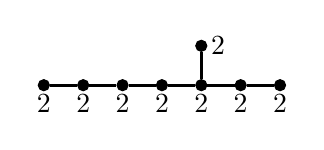
\begin{tikzpicture}
			\tikzset{dynode/.style={circle, draw, fill=black,
						minimum size=4pt, inner sep=0pt}}
			\tikzset{dyline/.style={line width=1pt}}
			\tikzset{dydash/.style={line width=1pt, dashed}}

			\begin{scope}[yshift=-10em, xshift=0]
				\node[dynode] (a1) at (0,0) {};
				\node[dynode] (a2) at (0.5,0) {};
				\node[dynode] (a3) at (1,0) {};
				\node[dynode] (a4) at (1.5,0) {};
				\node[dynode] (a5) at (2,0) {};
				\node[dynode] (a6) at (2.5,0) {};
				\node[dynode] (a7) at (3,0) {};
				\node[dynode] (a8) at (2,0.5) {};

				\draw[dyline] (a1) -- (a2) -- (a3) -- (a4) -- (a5) -- (a6) -- (a7);
				\draw[dyline] (a5) -- (a8);

				\node[below] () at (a1) {$2$};
				\node[below] () at (a2) {$2$};
				\node[below] () at (a3) {$2$};
				\node[below] () at (a4) {$2$};
				\node[below] () at (a5) {$2$};
				\node[below] () at (a6) {$2$};
				\node[below] () at (a7) {$2$};
				\node[right] () at (a8) {$2$};
			\end{scope}
		\end{tikzpicture}
		\quad\implies\quad
		\begin{pmatrix}
			2 & 1 &   &   &   &   &   &   \\
			1 & 2 & 1 &   &   &   &   &   \\
			  & 1 & 2 & 1 &   &   &   &   \\
			  &   & 1 & 2 & 1 &   &   &   \\
			  &   &   & 1 & 2 & 1 & 0 & 1 \\
			  &   &   &   & 1 & 2 & 1 & 0 \\
			  &   &   &   & 0 & 1 & 2 & 0 \\
			  &   &   &   & 1 & 0 & 0 & 2 \\
		\end{pmatrix}
	\]
	where each vertex of the tree is weighed by $2$.
\end{proposition}

It's interesting to note that if $Q$ is a matrix associated to a tree $T$, then $P(Q)$ has a $1$-skeleton homotopy equivalent to $T$. This connection between the $1$-skeleton and plumbing along a tree or graph was first noticed by Hirzebruch. It makes sense then why we'd care about matrices arising from trees instead of from general graphs which may contain cycles -- cycles break the simple-connectedness of the constructed manifold and are thereby much more complicated to work with.

% \begin{figure}[ht]\label{fig:negative-definite-trees}
% 	\centering
% 	\begin{tikzpicture}
% 		\tikzset{dynode/.style={circle, draw, fill=black,
% 					minimum size=4pt, inner sep=0pt}}
% 		\tikzset{dyline/.style={line width=1pt}}
% 		\tikzset{dydash/.style={line width=1pt, dashed}}
%
% 		\begin{scope}[yshift=0, xshift=22em]
% 			\node[dynode] (a1) at (0,0) {};
% 			\node[dynode] (a2) at (0.5,0) {};
% 			\node[dynode] (a3) at (1,0) {};
% 			\node[dynode] (a4) at (1.5,0) {};
% 			\node[dynode] (a5) at (2,0) {};
% 			\node[dynode] (a6) at (2.5,0) {};
% 			\node[dynode] (a7) at (3,0) {};
% 			\node[dynode] (a8) at (2,0.5) {};
%
% 			\draw[dyline] (a1) -- (a2) -- (a3) -- (a4) -- (a5) -- (a6) -- (a7);
% 			\draw[dyline] (a5) -- (a8);
%
% 			\node[] (l) at (1.75,-0.5) {$\E_8$};
% 		\end{scope}
%
% 		\begin{scope}[yshift=0, xshift=10em]
% 			\node[dynode] (a1) at (0,0) {};
% 			\node[dynode] (a2) at (0.5,0) {};
% 			\node[dynode] (a3) at (1,0) {};
% 			\node[dynode] (a4) at (1.5,0) {};
% 			\node[dynode] (a5) at (2,0) {};
% 			\node[dynode] (a6) at (2.5,0) {};
% 			\node[dynode] (a8) at (1.5,0.5) {};
%
% 			\draw[dyline] (a1) -- (a2) -- (a3) -- (a4) -- (a5) -- (a6);
% 			\draw[dyline] (a4) -- (a8);
%
% 			\node[] (l) at (1.5,-0.5) {$\E_7$};
% 		\end{scope}
%
% 		\begin{scope}[yshift=0, xshift=0]
% 			\node[dynode] (a1) at (0,0) {};
% 			\node[dynode] (a2) at (0.5,0) {};
% 			\node[dynode] (a3) at (1,0) {};
% 			\node[dynode] (a4) at (1.5,0) {};
% 			\node[dynode] (a5) at (2,0) {};
% 			\node[dynode] (a8) at (1,0.5) {};
%
% 			\draw[dyline] (a1) -- (a2) -- (a3) -- (a4) -- (a5);
% 			\draw[dyline] (a3) -- (a8);
%
% 			\node[] (l) at (1,-0.5) {$\E_6$};
% 		\end{scope}
%
% 		\begin{scope}[yshift=5em, xshift=3em]
% 			\node[dynode] (a1) at (0,0) {};
% 			\node[dynode] (a3) at (0.5,0) {};
% 			\node[dynode] (a4) at (1,0) {};
% 			\node[dynode] (a5) at (2.5,0) {};
% 			\node[dynode] (a6) at (3.0,0) {};
%
% 			\draw[dyline] (a1) -- (a3) -- (a4);
% 			\draw[dydash] (a4) -- (a5);
% 			\draw[dyline] (a5) -- (a6);
%
% 			\node[] (l) at (1.75,-0.5) {$\op{A}_n$};
% 		\end{scope}
%
% 		\begin{scope}[yshift=5em, xshift=17em]
% 			\node[dynode] (a1) at (0,0.4) {};
% 			\node[dynode] (a2) at (0,-0.4) {};
% 			\node[dynode] (a3) at (0.5,0) {};
% 			\node[dynode] (a4) at (1,0) {};
% 			\node[dynode] (a5) at (2.5,0) {};
% 			\node[dynode] (a6) at (3.0,0) {};
%
% 			\draw[dyline] (a1) -- (a3);
% 			\draw[dyline] (a2) -- (a3);
% 			\draw[dyline] (a3) -- (a4);
% 			\draw[dydash] (a4) -- (a5);
% 			\draw[dyline] (a5) -- (a6);
%
% 			\node[] (l) at (1.75,-0.5) {$\op{D}_n$};
% 		\end{scope}
% 	\end{tikzpicture}
% 	\vspace{1em}
% 	\caption{\todo{describe}}
% \end{figure}

\subsection{The Topology of Plumbed Manifolds}\label{sec:homotopy-type-plumbed}

In this section, we'll

\begin{proposition}
	If $\partial P^{2m}(Q)$ is a homotopy sphere then $Q$ is unimodular.
\end{proposition}

\begin{theorem}
	When $k>1$, $\partial P^{4k}(Q)$ is a homotopy sphere if and only if $Q$ is unimodular.
\end{theorem}


\begin{definition}
	The for $k>1$, the \defn{Milnor sphere} is the homotopy sphere $\partial P^{4k-1}(E_8)$.
\end{definition}

\subsection{Plumbing Constructions of 3-Manifolds}

Many of the results about the homotopy theory of plumbed manifolds in \cref{sec:homotopy-type-plumbed} only apply in dimensions $>4$. We can however still do the plumbing construction in $4$ dimensions, and it would be interesting to see what we get. In particular 

\todo{this section should be rewritten}

This $3$-manifold is known as (Poincar\'e) \defn{dodecahedral space} and has a beautiful geometric construction. We'll denote this space by $\mathscr{D}$. Aside from being a wonderful example of a non-Euclidean geometry, this space also was the first counter-example to an incorrect earlier form of the Poincar\'e hypothesised which stated that every homology $3$-sphere was also homeomorphic to the $3$-sphere. Much like exotic spheres are counter-examples to the smooth Poincar\'e hypothesis, in a similar vein the dodecahedral space can be thought of as a sort of ``proto exotic sphere'' serving as a counter-example to the ``proto Poincar\'e hypothesis''.

The classic construction of dodecahedral space $\mathscr{D}$ is due to Poincar\'e \todo{cite}. We begin by letting $\mathcal{D}\subset \R^3$ be a solid dodecahedron in three dimensional Euclidean space. The dodecahedron has 6 pairs of opposite pentagonal faces. Picking a clockwise spherical orientation on $\mathcal{D}$, we can glue together opposing faces with a minimal clockwise twist to line them up (see \cref{fig:dodecahedral_space_construction}). The resulting quotient space is a closed $3$-manifold, and this manifold is dodecahedral space $\mathscr{D}$.

\begin{figure}[ht]
	\centering
	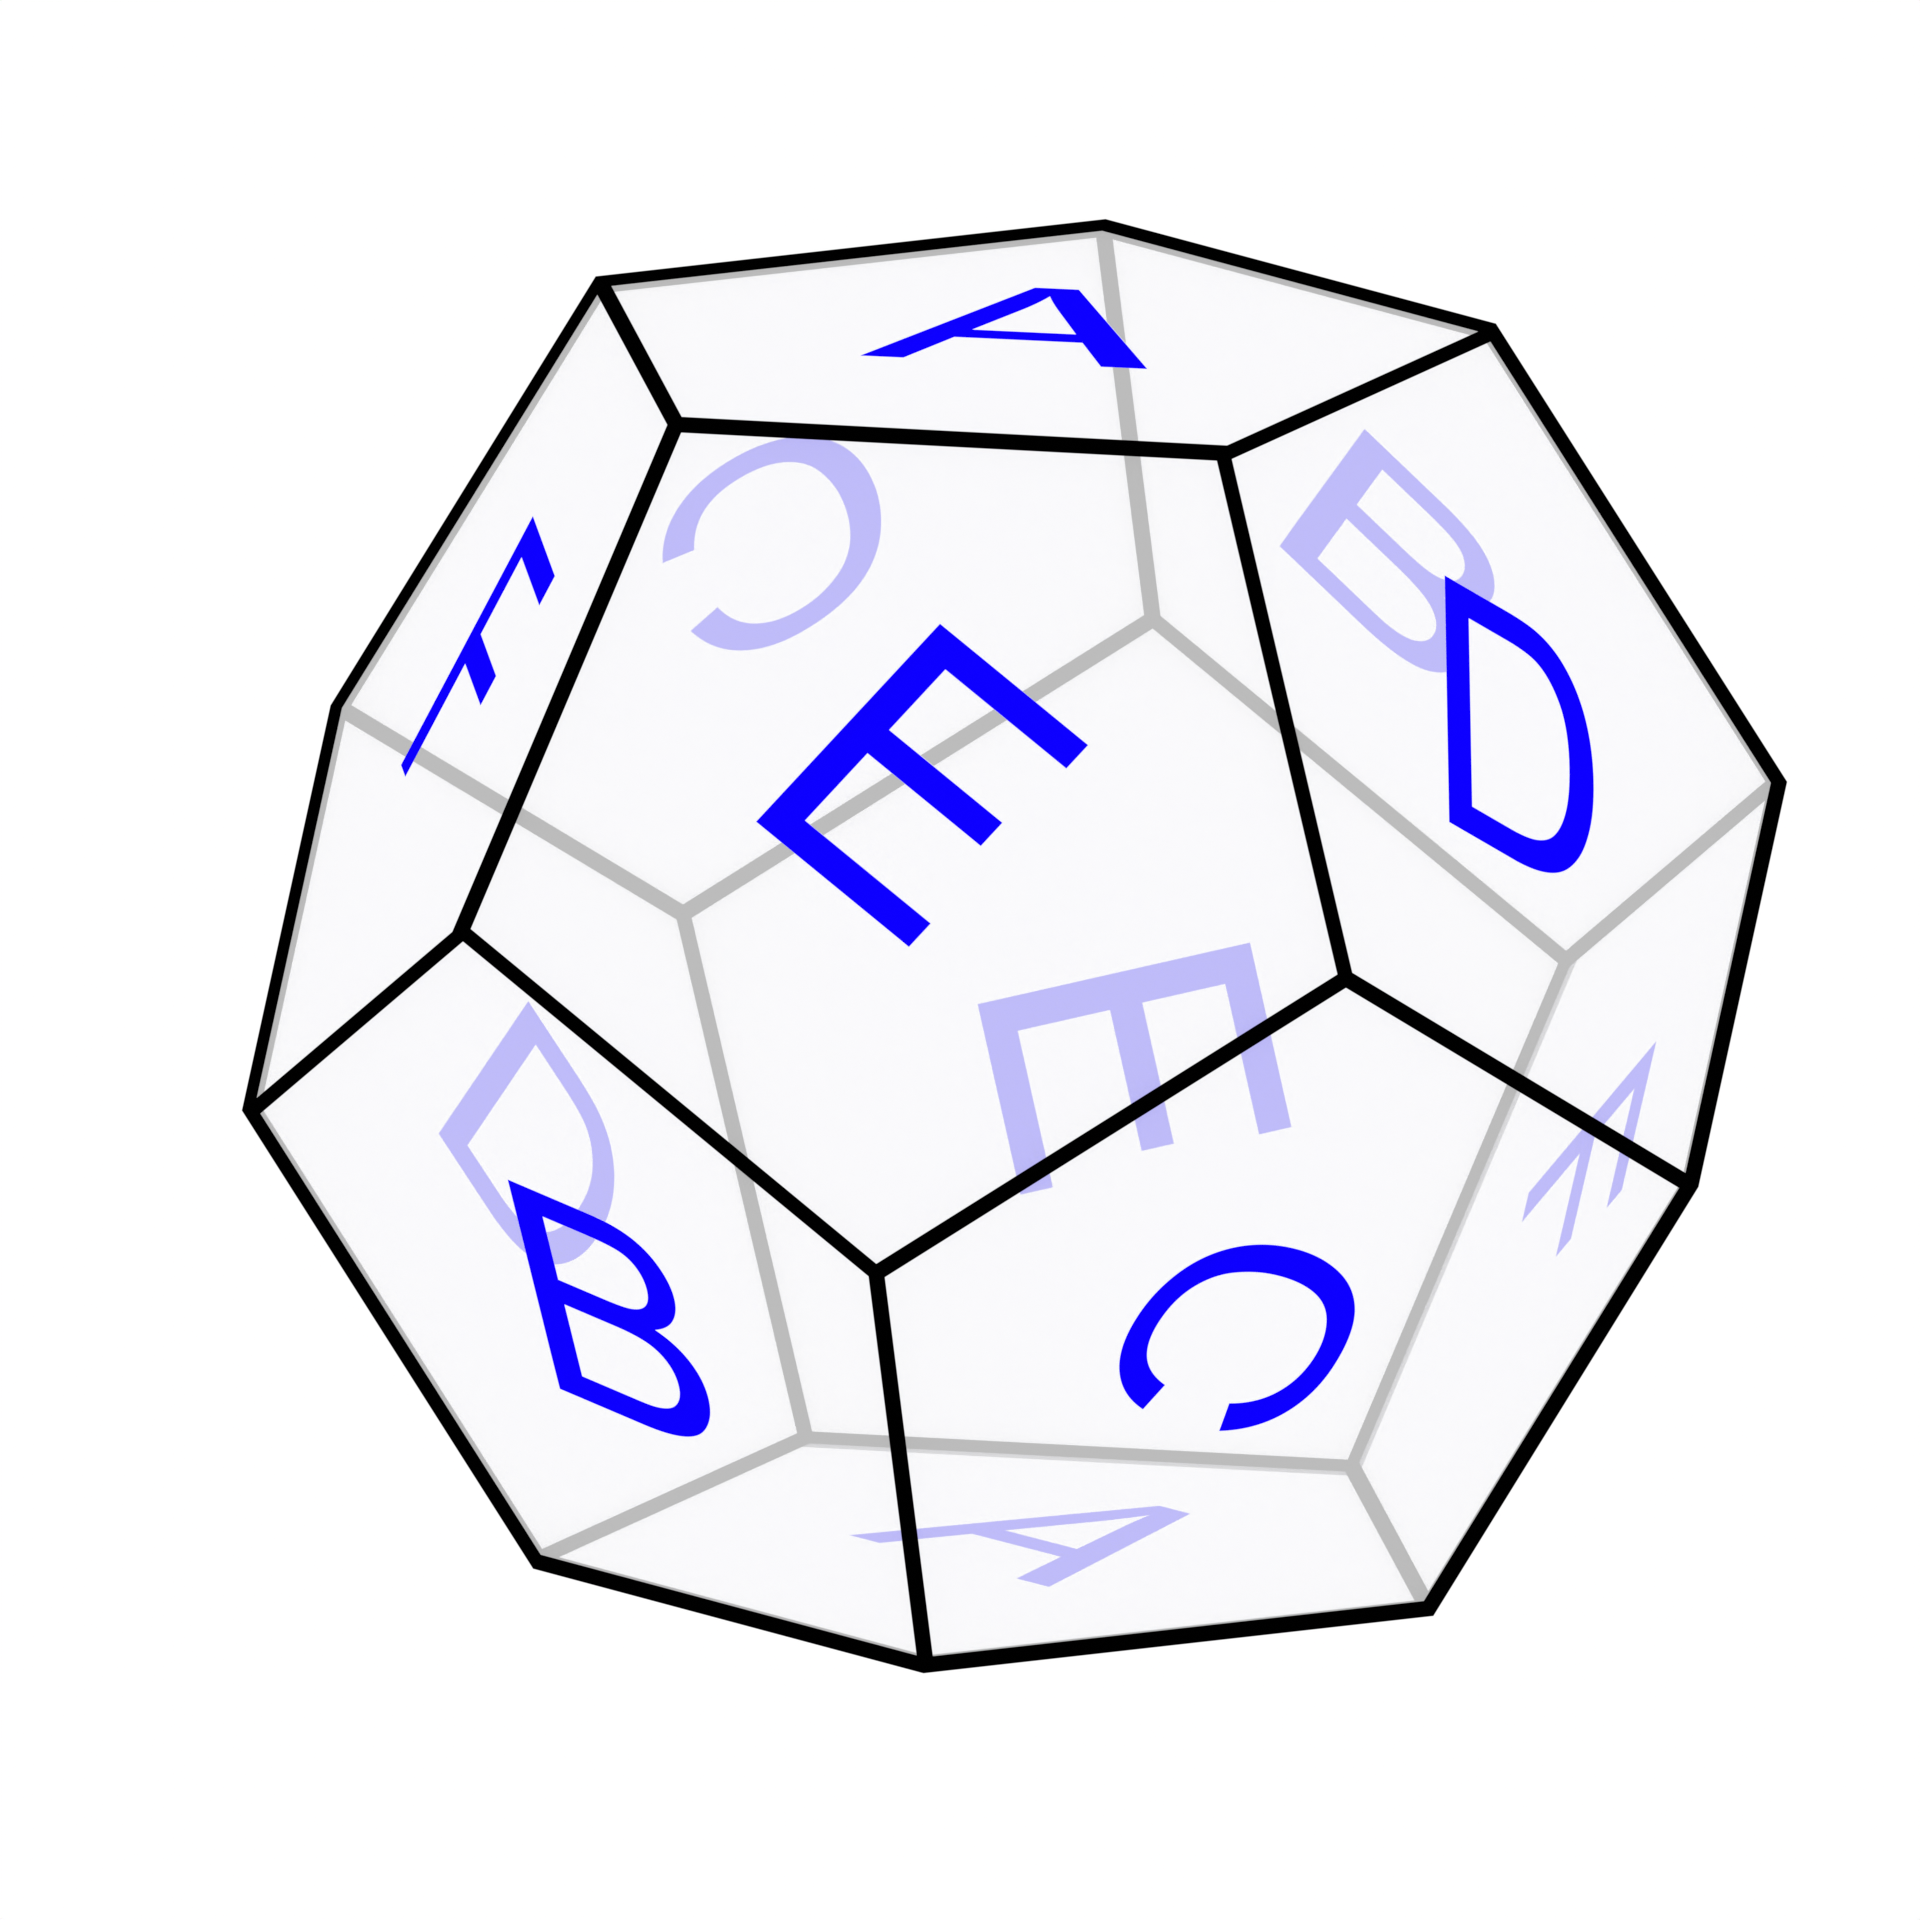
\includegraphics[width=2in]{graphics/temp-diagrams/dodecahedral-space-geometric-construction.png}
	\caption{Construction of Dodecahedral Space}\label{fig:dodecahedral_space_construction}
\end{figure}

Given this geometric construction, it should be fairly straightforward -- albeit tedious -- to compute the homology of dodecahedral space by means of a cellular decomposition. After such a computation, we would find that:
\begin{proposition}
	Dodecahedral space is a homology $3$-sphere.
\end{proposition}

While the first homology of dodecahedral space is trivial and incapable of differentiating dodecahedral space from a 3-sphere, the fundamental group reveals a much richer geometric structure. If we let $\SO_3$ act on $\R^3$ in the usual way, we can form the symmetry group $\Sym(\mathcal{D})\subset \SO_3$ of orientation preserving orthogonal transformations which leave the dodecahedron $\mathcal{D}$ unchanged. This is known as the \defn{icosahedral group}\footnote{The icosahedron and dodecahedron are dual, so the choice of icosahedral in the name is purely a historical convention.} $\mathrm{I}\subset \SO_3$, a group containing $60$ elements and isomorphic to the alternating group $A_5$. There is a double cover of $\SO_3$ by the $\Spin_3$ Lie group:
\[
	\SU_2\cong \Spin_3\lkxto[2:1] \SO_3
\]
The \defn{binary icosahedral group}, denoted $2\mathrm{I}$, is the preimage of $\mathrm{I}$ under this double cover and hence contains $120$ elements. Since there is an exceptional isomorphism $\SU_2\cong \Spin_3$, the binary icosahedral group admits a representation by unitary complex $2\times 2$ matrices.
We then have:
\begin{proposition}
	The fundamental group of dodecahedral space is the binary icosahedral group.
\end{proposition}
This hints at another interesting fact about the binary icosahedral group -- it is a \defn{perfect group}, which means that it's commutator subgroup is the entire group. By the Hurewicz isomorphism, it would follow that
\[
	\H_1(\mathscr{D}) \cong \Ab\left[ \pi_1(\mathscr{D})\right] \cong 2\mathrm{I}/[2\mathrm{I}, 2\mathrm{I}] = 0
\]
where $\Ab$ denotes the abelianization. This perfectness of the fundamental group thus ``hides'' the non-trivial topology of $\mathscr{D}$ from being detectable by homology. It's interesting to note that dodecahedral space and $S^3$ are the only homology $3$-spheres up to homeomorphism with finite fundamental groups.

There is also a useful construction of dodecahedral space which will later appear in our later study of Brieskorn manifolds in \todo{cite}. If we identify $\SU_2$ with the $3$-sphere of unit quaternions, we obtain the construction:

\begin{proposition}
	There is a diffeomorphism $\mathscr{D} \cong S^3 / 2\mathrm{I}$ expressing dodecahedral space as the quotient of the $3$-sphere under a proper group action by $2\mathrm{I}$.
\end{proposition}

Finally, let's see how the dodecahedral space and binary icosahedral group arises out of the plumbing construction we've worked with thus far.

\todo{write this section}

\begin{proposition}
	There is a diffeomorphism $\mathscr{D}\cong \partial P^4(\E_8)$.
\end{proposition}

\todo{citations}

\begin{remark}
	In the early 2000's, the Wilkinson Microwave Anisotropy Probe (WMAP) was launched to accurately map out the cosmic microwave background, i.e. leftover heat from the Big Bang. The observed lack of temperature correlations above 60$^\circ$ led astrophysicist Jean-Paul Luminet to propose a cosmological model \cite{luminet2003dodecahedral} where the shape of the universe is a dodecahedral space, explaining the lack of large scale correlations by means of the compact topology of space. In such a finite universe, larger temperature correlations simply wouldn't have enough room to form.
	While this model made some predictions aligning with observed cosmological data
	\cite{roukema2008dodecahedral}, higher resolution data by the later Planck spacecraft later seemed to suggest that the observable large scale topology is trivial, leading to the modern prevalence of the $\Lambda$CDM model as a standard model for cosmology.
\end{remark}

\section{Surgery Theory}

Now that we have the basic constructions out of the way, let's \todo{introduce}

\subsection{Groups of Homotopy Spheres}

\begin{definition}
	\todo{groups of homotopy spheres}
\end{definition}

\subsection{Fundamental Theorems of Surgery}

\begin{definition}
	\todo{surgical invariant $\sigma$}
\end{definition}

\begin{theorem}[Plumbing Theorem]\label{thm:plumbing-theorem}
	When $m>2$, there is a normal map \[(g,c) : (W,\partial W) \to (D^{2m}, S^{2m-1})\] which restricts to a homotopy equivalence $g|_{\partial W} : \partial W \to  S^{2m-1}$ with the invariant $\sigma(g,c)$ taking on any integer value.
\end{theorem}

% \section{Complex Singularities}
%
% Let $F\in \C[z_0,z_1\ldots, z_n]$ be a non-constant polynomial in $(n+1)$-complex variables.
% \begin{definition}
% 	The \defn{variety} of $F$ is the complex hypersurface given by the zero locus
% 	\[
% 		\V(F) = F^{-1}(0)=\left\{ z \in \C^{n+1}  F(z)=0\right\} \subset \C^{n+1}.
% 	\]
% \end{definition}
%
% \todo{cauchy riemann equations}
%
% \begin{definition}
% 	The \defn{gradient} of a complex analytic function $F : \C^{n+1} \to \C$ is the $(n+1)$-tuple
% 	\[
% 		\nabla_F = \left(\frac{\partial F}{\partial z_0}, \frac{\partial F}{\partial z_1},\ldots, \frac{\partial F}{\partial z_n}\right).
% 	\]
% 	\todo{better definition}
% \end{definition}
%
% \begin{definition}
% 	A point $w\in \V(F)$ is a (complex) \defn{singularity}[complex singularity] if $\nabla_F(w)$ vanishes. A singularity is \defn{isolated}[isolated singularity] if there is a neighborhood surrounding $w$ which contains no other singularities.
% \end{definition}
%
% \begin{theorem}
% 	For small $\varepsilon>0$ the intersection of $\V(F)$ with $D_\varepsilon(w)$
% \end{theorem}
%
% \begin{proposition}
% 	Every sufficiently small sphere around an isolated singularity of $F$ intersects $\V(F)$ transversally in a smooth manifold.
% \end{proposition}
%
% \begin{definition}
% 	Let $w\in \V(F)$ be an isolated singularity. The \defn{link} of $F$ at $w$ is the intersection
% 	\[
% 		\L(F, w) = \V(F) \cap S^{2n+1}_\varepsilon(w) = \left\{ z\in \C^{n+1}  F(z)=0\textrm{ and } |z-w|<\varepsilon\right\}
% 	\]
% 	where $\varepsilon > 0$ is some sufficiently small real number so that $\L(F,w)$ is a smooth manifold intersecting the sphere $S^{2n+1}_\varepsilon(w)$ transversally.
% \end{definition}
%
% When the isolated singularity is clear, we write $\L(F)$.
%
% \subsection{Brieskorn Manifolds}
% The simplest examples of complex polynomials with isolated singularities are \todo{this}
%
% \begin{definition}
% 	Let $(a_0,a_1,\ldots, a_n)$ be an $(n+1)$-tuple of integers greater than or equal to $2$. The \defn{Brieskorn polynomial} of the tuple $(a_0,a_1,\ldots, a_n)$ is given by
% 	\[
% 		F(z_0,z_1,\ldots, z_n) = z_0^{a_0} + z_1^{a_1} +\cdots + z_n^{a_n}.
% 	\]
% 	Correspondingly, we refer to $\V(F)$ as the \defn{Brieskorn variety} of the tuple and to the link at the origin $\L(F,0)$ origin as the \defn{Brieskorn manifold}. We'll use the notation
% 	\[
% 		\Sigma(a_0,a_1,\ldots, a_n) =\L(z_0^{a_0}+z_1^{a_1}+\cdots+z_n^{a_n}, 0)
% 	\]
% 	to refer to these Brieskorn manifolds.
% \end{definition}
%
%
% \begin{proposition}
% 	If $p,q\geq 2$, then $\Sigma(p,q)\subset S^3$ is the torus link of type $(p,q)$.
% \end{proposition}
%
% \begin{proposition}
% 	There is a homeomorphism $\Sigma(2,2,2)\cong \RP^3$.
% \end{proposition}
%
% \begin{proposition}
% 	There is a homeomorphism $\Sigma(2,3,5)\cong \mathscr{D}$.
% \end{proposition}
%
% \subsection{The Fibration Theorem}
%
% \begin{theorem}\label{thm:fibration}
% 	If $F$ is a complex polynomial in $(n+1)$-variables with an isolated singularity at the origin, then there is a smooth fiber bundle map
% 	\[
% 		\lkxfunc{\phi}{S^{2n+1}_\varepsilon - \L(F)}{S^1}{z}{\arg F(z).}
% 	\]
% \end{theorem}
%
% For a given angle $e^{i\theta}\in S^1$, we'll denote the fiber of the bundle $\phi$ as $F_\theta = \phi^{-1}(e^{i\theta})$.
%
% \begin{proposition}
% 	Each fiber $F_\theta$ is a smooth parallelizable $2n$-manifold.
% \end{proposition}
%
% \subsection{When is the link a topological sphere?}
%
% Let's fix a polynomial $F$ in $(n+1)$ complex variables
%
% \begin{proposition}
% 	If $n\neq 2$, then $\L$ is homeomorphic to the sphere $S^{2n-1}$ if and only if $\L$ has the homology of a sphere. In fact, $\L$ is a topological sphere if and only if the reduced homology $\widetilde{H}_{n-1}(\L)$ is trivial.
% \end{proposition}
%
% Let's now choose an orientation for $F_\theta$.
%
% \begin{proposition}
% 	The manifold $\L$ is a homology sphere if and only if the intersection form
% 	\[
% 		\lkxfunc{Q_{F_\theta}}{\H_n(F_\theta)\times \H_n(F_\theta)}{\Z}
% 	\]
% 	has determinant $\pm 1$ -- in other words if $Q_{F_\theta}$ is unimodular.
% \end{proposition}
%
% \section{Kervaire Invariant}
%
% \begin{theorem}[Brieskorn-Pham]
% \end{theorem}
%
% \begin{theorem}[Levine]
% 	If $n$ is odd, the Kervaire invariant is given by
% 	\[
% 		c(F_0) = \begin{cases}
% 			0 & \textrm{if }\Delta(-1)\equiv \pm 1\mod 8 \\
% 			1 & \textrm{if }\Delta(-1)\equiv \pm 3\mod 8
% 		\end{cases}
% 	\]
% \end{theorem}
%
% \begin{theorem}[Hirzebruch-Mayer] Smooth Brieskorn varieties are parallelizable.
% \end{theorem}


\chapter{Classification of Homotopy Spheres}\label{chap:classification}
\chapter{Classification}\label{chap:classification}

\begin{epigraph}{8.6em}{David Hilbert}
	Wir w\"ussen wissen.\\
	Wir werden wissen.
\end{epigraph}

In this penultimate chapter, we will prove general theorems about the group $\Theta^n$ of smooth structures on the sphere, in some respects, a full classification depending on the solutions of problems in homotopy theory. As we have discussed in \cref{sec:groups-of-homotopy-spheres}, there are generally two classes of exotic spheres -- those that bound parallelizable manifolds, i.e. $\bP^{n+1}\subset \Theta^n$, and those that do not, i.e. $\Theta^n/\bP^{n+1}$.
Exotic spheres represented by the latter set are known as \defn{very exotic spheres}, and are far harder to construct or visualize since they can only really be detected by homotopy theoretic means.
We have seen how to construct exotic spheres in $\bP^{n+1}$ in \cref{chap:constructions}, and have even computed divisibility lower bounds on the size of $\bP^{4k}$ using geometric invariants in \cref{chap:invariants}. We will now
\begin{itemize}
	\item prove that $\bP^{4k}$ is a cyclic group and derive a formula for its order (\cref{thm:kervaire-milnor}), making exact the lower bounds of \cref{chap:invariants},
	\item prove that the groups $\bP^{4k+2}$ are either trivial or $\Z/2$ depending on the Kervaire invariant problem (\cref{thm:kervaire-invariant-problem}),
	\item prove that the groups $\bP^{2k+1}$ are trivial (\cref{cor:odd-dimensional-bP-trivial}),
	\item prove that $\Theta^n/\bP^{n+1}$ are finite groups (\cref{thm:finite-very-exotic-spheres}) and consequently $\Theta^n$ are finite,
	\item relate the quotient $\Theta^n/\bP^{n+1}$ of very exotic spheres to the $J$-homomorphism and the stable homotopy groups of spheres.
\end{itemize}
Altogether, these results

Many of these results fit into an 

\pagebreak
\section{Homotopy Theory and Geometry}

homotopy theory can act as a ``moduli space'' for geometric problems. The familiar example of this is the case of vector bundles, where we caught a glimpse of the geometric insights which can be provided by homotopy theory in the construction of the universal bundle and universal characteristic classes. There, we saw that up to isomorphism, vector bundles were completely classified by a set of homotopy classes of map.
In this section, we will apply a similar principle to manifolds themselves, relating various notions of cobordism to homotopy groups of spectra.

\subsection{The Thom-Pontryagin Construction}

Let us begin with the classical theory for framed cobordism, originally due Pontryagin in 1950 (see \cite{pontryagin1959homotopy} for a translation of a thorough exposition by Pontryagin). 

The basic idea is simple and geometric. Suppose we have closed ambient manifold $M^n$ with submanifold $N^k$ possessing a tubular neighborhood $T_N\supset N$. Recall that a framing on $N$ is a diffeomorphism $\varphi : T_N \to N\times \R^{n-k}$. If we project onto the second factor, we get a map $\varphi'=\pi_2\circ \varphi : T_N \to \R^{n-k}$. We can then include $\R^{n-k}$ into its one-point compactification $\R^{n-k}\cup \{\infty\}=S^{n-k}$ by stereographic projection, and extend the map $\varphi'$ to $S^{n-k}$ by sending $N\setminus T_N$ to $\infty$. We can associate this map $f : M \to S^{n-k}$ to the framed embedding $N\subset M$.
\[\begin{tikzcd}
	N & {T_N} & M \\
	{\{0\}} & {\R^{n-k}} & {S^{n-k}}
	\arrow[hook, from=1-1, to=1-2]
	\arrow[from=1-1, to=2-1]
	\arrow[hook, from=1-2, to=1-3]
	\arrow["{\varphi'}", from=1-2, to=2-2]
	\arrow["f", from=1-3, to=2-3]
	\arrow[hook, from=2-1, to=2-2]
	\arrow[hook, from=2-2, to=2-3]
\end{tikzcd}\]

This construction is not too surprising, $N$ is sent to the point $0\in S^{n-k}$, and $M\setminus T_N$ is sent to the $\infty \in S^{n-k}$ (although any distinct pair of points would suffice). The tubular neighborhood fills in the gaps, encoding the ``twistedness'' of the framing of $N\subset M$ in the homotopy type of the map $f$.

\begin{proposition}
	The map $f$ is smooth, and $0\in S^{n-k}$ is a regular value.
\end{proposition}

\begin{figure}[ht]
	\import{diagrams}{placeholder.pdf_tex}
	\caption{Turning a framed submanifold of $M$ into a map $M\to S^{n-k}$.}
\end{figure}

In the reverse direction, suppose we had a smooth map $f : M \to S^{n-k}$ with 

\begin{definition}
	If $N_1$ and $N_2$ are embedded submanifolds of $M$, a \defn{framed cobordism in $M$}[framed cobordism] $W : N_1 \frbord{M} N_2$ of $N_1$ and $N_2$ is a framed submanifold $W\subset M\times [0,1]$ such 
\end{definition}

\begin{definition}
	The group of framed cobordism classes of framed $k$-dimensional submanifolds of $M$ is denoted $\Omega^\fr_k(M)$.
\end{definition}

A good example and source of intuition for this construction comes from framed knots. In knot theory, a \defn{framed knot} is an embedding $\iota$ of $S^1$ into $S^3$ along with a section $s$ of its normal bundle $\T S^3/S^1$. A framed knot should be thought of as an embedded ``ribbon'' in three dimensional space, the underlying knot determining the knottedness of the ribbon and the framing section determining the twistedness of the ribbon. For some examples of framed knots, see \cref{fig:framed-knot-examples}.

\begin{figure}[ht]
	\centering
	\import{diagrams}{placeholder.pdf_tex}
	\caption{A framed unknot and trefoil knot.}\label{fig:framed-knot-examples}
\end{figure}

\begin{remark}
With a Riemannian structure on $S^3$, we can assume without loss of generality that $s$ has unit norm, and get an orthonormal section $s^\perp$ to $s$. This recovers our notion of a framed submanifold, since $s\oplus s^\perp$ defines trivializations for a tubular neighborhood of the (unframed) knot $\iota(S^1)$ in $S^3$.
\end{remark}

Under the construction described above, a framed knot corresponds to a map $f : S^3\to S^{2}$.
\todo{self-linking}

\begin{theorem}[Pontryagin Isomorphism]\label{thm:thom-pontryagin-isomorphism}
	Given a closed manifold $M^n$ of dimension $n>k$, there is a bijective correspondence
	\begin{equation}
		\lkxfunc{p^\fr_k(M)}{\Omega^\fr_k(M)}{{}[M, S^{n-k}].}
	\end{equation}
\end{theorem}

\subsection{Stable Homotopy Theory}

\begin{definition}
	The \defn{stable homotopy groups} of a pointed space $X$ are the colimits
	\[
		\pi_n^{s}(X) = \varinjlim_k \pi_{n+k}(\Sigma^k X).
	\]
\end{definition}

\begin{definition}
	The susepsnion 
\end{definition}

\begin{definition}
	The \defn{sphere spectrum} is the suspension spectrum of the point.
\end{definition}

\begin{theorem}[Stable Pontryagin Isomorphism]
	There is a group isomorphism
	\[
		\lkxfunc{p^\fr_k}{\Omega_k^\fr}{\pi_k(\mathcal{S})}
	\]
\end{theorem}

\subsection{Obstruction Theory}

\pagebreak
\section{Framed Surgery Theory}

In \cref{sec:plumbing} and \cref{sec:brieskorn}, we constructed highly-connected manifolds

\begin{theorem}\label{thm:framed-surgery-highly-connected}
  Every compact framed manifold of dimension $n\geq 4$ with boundary $\partial M$ a homology sphere can be made highly-connected by a finite sequence of framed surgeries.
\end{theorem}

This is a bulky theorem, and so we will tackle it in parts. First, let us understand the effect of 

\begin{proof}
\end{proof}

\begin{corollary}\label{cor:odd-dimensional-bP-trivial}
	The groups $|\bP^{2k+1}|$ are trivial.
\end{corollary}

\subsection{The Surgery Invariant}\label{sec:surgery-invariant}

\begin{theorem}[Milnor-Kervaire]\label{thm:kervaire-milnor}
	For every $k>1$, $bP^{4k}$ is a cyclic group of order
	\[
	  |\bP^{4k}| =2^{2k-2}(2^{2k-1}-1)\epsilon(k)\denom(4k/B_{2k}).
	\]
\end{theorem}

\begin{theorem}[Kervaire Invariant Problem]\label{thm:kervaire-invariant-problem}
\end{theorem}

\begin{theorem}\label{thm:homotopy-sphere-stably-parallelizable}
	Every homotopy sphere is stably parallelizable.
\end{theorem}
\begin{proof}
	Let $\Sigma$ be a homotopy $n$-sphere.

	The only obstruction to the triviality of $T^sM$ is a well-defined cohomology class:
	\[
		\mathfrak{o}_n(\Sigma) \in \H^n(\Sigma; \pi_{n-1}(\SO_{n+1})) = \pi_{n-1}(\SO_{n+1})
	\]
	The coefficient group may be identified with the stable group $\pi_{n-1}(\SO)$, but these stable groups have been computed by Bott in \cite{bott1959stable}, for $n\geq 2$ we have:
	\begin{center}
		\begin{tabular}{c|cccccccc}
			\textrm{$n\mod 8$} & 0 & 1 & 2 & 3 & 4 & 5 & 6 & 7\\
			\hline
			$\pi_{n-1}(\SO)$ & $\Z$ & $\Z/2$ & $\Z/2$ & 0 & $\Z$ & 0 & 0 & 0.
		\end{tabular}
	\end{center}
	If $\pi_{n-1}(\SO)$ is zero, we are done. 

	If $\pi_{n-1}(\SO) = \Z$, then $n=4k$. According to cite{kervairemilnor1960} and cite{kervaire1959}, some non-zero multiple of the obstruction class $\mathfrak{o}_n(\Sigma)$ can be identified with the Pontryagin class $p_k(T^s M) = p_k(TM)$. \todo{(why?)} But the Hirzebruch signature theorem implies \todo{(why?)} that $p_k(\Sigma)$ is a multiple of the signature $\sigma(\Sigma)$ which is zero since $\H^{2k}(\Sigma)=0$. Thus every homotopy $4k$-sphere is \textsc{s}-parallelizable. 

	Finally, suppose $\pi_{n-1}(\SO)= \Z_2$. It follows from an argument of Rohlin \todo{(what?)} that $J_{n-1}(\mathfrak{o}_n(\Sigma))=0$ where $J_{n-1}$ denotes the Hopf-Whitehead homomorphism
	\[
		\lkxfunc{J_{n-1}}{\pi_{n-1}(\SO_k)}{\pi_{n+k-1}(S^k)}
	\]
	in the stable range $k >n$. But $J_{n-1}$ is injective for $n\equiv 1, 2\mod 8$. This is proven by Adams. \todo{(find)} This means that $\mathfrak{o}_n(\Sigma)=0$.
\end{proof}

\section{Very Exotic Spheres}

\begin{theorem}\label{thm:finite-very-exotic-spheres}
	The quotient group $\Theta^n / \bP^{n+1}$ is finite.
\end{theorem}
\begin{proof}
	Let $M$ be an \textsc{s}-parallelizable $n$-manifold. 

	Imbed it as $i : M \to S^{n+k}$ for some $k>n+1$ so that it's normal bundle is trivial.

	For each normal $k$-frame $\varphi$, we get an element of $\pi_{n+k}(S^k) = \pi^s(S^n)$ by the Pontryagin-Thom construction. Let's call the set of these elements (as $\varphi$ is allowed to vary) $p(\Sigma)$. \todo{(elaborate)}

	\todo{add lemmas}

	\begin{lemma}
		There is a homomorphism:
		\[
			\lkxfunc{p'}{\Theta_n}{\pi^s(S^n)/p(S^n)}
		\]
	\end{lemma}

	Furthermore, the kernel of $p'$ contains $h$-cobordism classes of homotopy $n$-spheres which bound parallelizable manifolds \todo{(provide lemma)}, which is exactly $bP_{n+1}$. By the first isomorphism theorem, it follows that $\Theta_n/bP_{n+1}$ is isomorphic to a subgroup of $\pi^s(S^n)$ which is finite.
\end{proof}

\subsection{Obstruction Theory}\label{sec:obstruction-theory}

% \section{Kervaire Invariant}


\begin{appendices}
\chapter{Differential Geometry}\label{chap:differential_geometry}
\begin{flushleft}
	\textsl{I admire the elegance of your method of computation;}\\
	\textsl{it must be nice to ride through these fields upon the}\\
  \textsl{horse of true mathematics while the like of us have to}\\
  \textsl{make our way laboriously on foot.}\\
	\rule[0pt]{24em}{0.5pt}\\
	-- \textsc{Albert Einstein} to \textsc{Tullio Levi-Civita}\\
	\vspace{2em}
\end{flushleft}

\begin{definition}\label{defn:manifold_structure}
  Let $(G,\rho)$ be an $n$-dimensional symmetry type and suppose $X$ is an $n$-dimensional manifold with frame bundle $\varpi : \B X \to X$. A \defn{$(G,\rho)$-structure} on $X$ is a reduction of $\varpi$ along the representation $\rho : G \to \GL_n$.
\end{definition}

\section{Lie Groups and Lie Algebras}

\section{Connections on Principal Bundles}


\chapter{Characteristic Classes}\label{chap:characteristic_classes}
% \section{The Chern-Weil Homomorphism}

\begin{definition}\label{defn:poincare-pair}
	Let $X$ be an $n$-dimensional manifold and $Y$ a closed submanifold. The pair $(X,Y)$ is said to be a \defn{Poincar\'e pair} if there is a fundamental class $[X, Y]\in \H_n(X,Y)$ such that the map
	\[
		\lkxfunc{}{\H^q(X,Y)}{\H_{n-q}(X)}{\omega}{\omega \frown [X, Y]}
	\]
	given by cap product with the fundamental class is an isomorphism.
\end{definition}

\begin{remark}\label{rmk:duality-integration}
In the case of de Rham cohomology, since $X$ is connected we have $\H_0(X)\cong \R$. Under this identification, the Poincar\'e duality isomorphism for top-dimensional relative cohomology classes $\omega\in \H^n(X,Y)$ can be interpreted as integration, i.e. $\omega\frown [X,Y]$ corresponds to $\int_X \omega$. 
\end{remark}

With this notion of a Poincar\'e pair, the classical statement of Poincar\'e duality is given:

\begin{theorem}[Poincar\'e Duality]\label{thm:poincare-duality}
	If $X$ is a closed manifold, then $(X,\emptyset)$ is a Poincar\'e pair.
\end{theorem}

\begin{theorem}[Poincar\'e-Lefschetz Duality]\label{thm:poincare-lefschetz-duality}
	If $X$ is a compact manifold with boundary, then $(X,\partial X)$ is a Poincar\'e pair.
\end{theorem}

\[
	\delta I = \int_X \omega + d\mathcal{A} - \int_X \omega =\int_X d\mathcal{A} =\int_{\partial X} \mathcal{A}
\]

\begin{definition*}
	A \defn{characteristic class} is a natural transformation 
	\[
		\lkxfunc{c}{\Bun_{G}}{h^\bullet}
	\]
	from the set of principal $G$-bundles
\end{definition*}

One of the fundamental topological invariants of a $2m$-manifold is its intersection form, a bilinear form which ``counts'' the number of intersections of submanifolds. We'll see this geometric interpretation in \cref{chap:construction_a}, but for now we'll stick to a more algebraic definition.

\begin{definition}\label{defn:intersection-form}
	Let $(X,Y)$ be a Poincar\'e pair where $X$ is a $2m$-manifold. The \defn{intersection form} of $(X,Y)$ is the bilinear form on $\H^{m}(X,Y)$ given by
	\[
		\lkxfunc{}{\H^{m}(X,Y)^{\times 2}}{\R}{\alpha, \beta}{(\alpha\smile\beta)[X,Y]}
	\]
	where $[X,Y]\in \H_{2m}(X,Y)$ is an orientation class.
\end{definition}
By the graded-commutativity of the cap product, when $m$ is odd this form is skew-symmetric and when $m$ is even this form is symmetric. For now, let's assume $m$ is even so that the form is symmetric bilinear. Following our conventions, we'll now write $2m=4k$. 


\section{Chern and Pontryagin Classes}

\begin{proposition}\label{prop:pontryagin_classes_of_CPn}
  The Pontryagin classes of complex projective space $\CP^n$ are
  \[
    p_k(\CP^n) = \binom{n+1}{k}\quad\textrm{for}\quad 1\leq k \leq n/2.
  \]
\end{proposition}

\section{Stiefel-Whitney Classes}\label{sec:stiefel-whitney_classes}

\section{Universal Bundles}\label{sec:universal_bundles}

\todo{"the most twisted bundle" from Bott and Tu}
\cite{milnorstasheff1974characteristic}
\cite{botttu1982differential}

\begin{theorem}\label{thm:cohomology_of_BO}
  There is a ring isomorphism
  \[
    \H^\bullet(\BO_n; \Z/2) \cong \Z/2[w_1,\ldots, w_n]
  \]
  where $w_i$ are Stiefel-Whitney classes of the universal bundle over $\BO_n$. In other words, any characteristic class for unoriented real bundles with $\Z/2$-coefficients can be expressed in terms of the Stiefel-Whitney classes.
\end{theorem}

\begin{theorem}\label{thm:cohomology_of_BSO}
  Let $\Lambda$ be an integral domain containing $1/2$. There are ring isomorphisms
  \[
      \H^\bullet(\BSO_{2m+1}; \Lambda) \cong \Lambda[p_1, \ldots, p_m]
      \quad\textrm{and}\quad
      \H^\bullet(\BSO_{2m}; \Lambda) \cong \Lambda[p_1, \ldots, p_m, e]/(e^2-p_m)
  \]
  where $p_i$ and $e$ are Pontryagin and Euler classes of the universal bundle over $\BSO_n$.
  In other words, ignoring $2$-torsion, any characterstic class for oriented real bundles can be expressed in terms of Pontryagin and Euler classes.
\end{theorem}

\section{Intersection Form}


\chapter{Cobordism}\label{chap:cobordism}
\section{Thom-Pontryagin Construction}\label{sec:thom-pontryagin_construction}

\section{The Rational Oriented Cobordism Ring}

\begin{theorem}[Thom-Pontryagin]\label{thm:thom-pontryagin_oriented_cobordism}
  The following holds:
  \begin{enumerate}
    \item There is a ring isomorphism $\Omega^\SO_\bullet \cong \pi_\bullet \MSO$.
    \item There is a ring isomorphism $\pi_\bullet\MSO \otimes \Q \cong \H_\bullet(\BSO; \Q)$.
    \item We have $\H_\bullet(\BSO; \Q) \cong \Q[p_1, p_2,\ldots]$ where $|p_i|=4i$.
  \end{enumerate}
  Putting this all together, there is a ring isomorphism
  \[
    \Omega^\SO_\bullet\otimes \Q \lkxto[\cong] \Q[[\CP^2], [\CP^4],\ldots]
  \]
  where $[\CP^{2n}]$ are oriented cobordism classes of complex projective planes.
\end{theorem}


\chapter{Index Theory}\label{chap:index_theory}

\section{The Hirzebruch Signature Theorem}

\begin{theorem}[Hirzebruch Signature Theorem]\label{thm:hirzebruch_signature}
  \todo{todo}
\end{theorem}

\section{The Atiyah-Singer Index Theorem}

\begin{theorem}[Atiyah-Singer Index Theorem]\label{thm:atiyah-singer_index}
  Let $X$ be a closed oriented $n$-manifold and let $(E,D)$ be an elliptic complex on $X$. Then we have
  \[
    \ind D = (-1)^{n(n+1)/2}\int_X \mathrm{ch}(E,D)\smile \Td(\T X_\C).
  \]
\end{theorem}


\chapter{Homotopy Groups of Spheres}\label{chap:homotopy_groups_of_spheres}
\input{chapters/homotopy_groups_spheres}
\end{appendices}

\lkxrefs
\lkxindex

\end{document}
